% Target journal: Entropy (MDPI), section "Information Theory, Probability and Statistics".
% Back matter below follows MDPI's required heading set and order (Author Contributions,
% Funding, IRB Statement, Informed Consent Statement, Data Availability Statement,
% Acknowledgments, Conflicts of Interest). Not yet converted to the mdpi.cls template.
\documentclass[11pt]{article}

\usepackage[T1]{fontenc}
\usepackage[utf8]{inputenc}
\usepackage{amsmath,amssymb,amsthm}
\usepackage[numbers,square,sort&compress]{natbib}
\usepackage{tabularx}
\usepackage{booktabs}
\usepackage{multirow}
\usepackage{float}
\usepackage{tikz}
\usepackage{pgfplots}
\pgfplotsset{compat=1.18}
\usepackage[margin=1in]{geometry}
\usepackage{graphicx}
\usepackage[colorlinks=true,linkcolor=blue,citecolor=blue,urlcolor=blue]{hyperref}

\newcolumntype{C}{>{\centering\arraybackslash}X}

\newtheorem{Definition}{Definition}
\newtheorem{Proposition}{Proposition}
\newtheorem{Theorem}{Theorem}
\newtheorem{Corollary}{Corollary}
\newtheorem{Remark}{Remark}
\newtheorem{Example}{Example}
\newtheorem{Assumption}{Assumption}

\title{Fisher-Information Feature Selection for Breast-Cancer Data Mining and Ill-Posed Inverse Problems: D-Optimal Design, Random-Matrix Denoising, and Entropy, with a Spectral Reflectance Case Study}
\author{Cesar Galindo\thanks{Corresponding author: jcgalindo@up.edu.mx}\\
\small Facultad de Empresariales, Universidad Panamericana, Ciudad UP, Mexico City 03920, Mexico\\
\small \texttt{cgalindo@up.edu.mx}}
\date{}

\begin{document}

\maketitle

\begin{abstract}
\noindent Fixed-budget feature selection is a standard data-mining problem in computational genomics: given a candidate library of probes or genes and a learned low-dimensional representation of a phenotype, which fixed-size subset should be measured? Breast-cancer subtyping and prognosis pose this problem directly. The 21-gene Oncotype DX recurrence score, the 70-gene MammaPrint signature, and the 50-gene PAM50 classifier are three clinically established, separately derived answers to it. The same literature uses, separately, mutual-information feature selection (mRMR, MIFS), random-matrix-theory (RMT) thresholding of gene co-expression networks, and wavelet denoising of copy-number and expression data. None of these is a design criterion in the classical experimental-design sense of maximizing information subject to a measurement budget. This paper supplies that criterion: D-optimal design, maximizing the determinant of the Fisher information matrix induced by a learned latent basis. We prove five structural results for it --- a rank-monotonicity proposition, an exact degeneracy characterization, an AM--GM inequality linking D- to A-optimality, a quantitative E-optimality guarantee, and an exact identification with maximum expected Shannon information gain in the weak-prior limit --- and derive and Monte-Carlo-verify the Poisson and negative-binomial Fisher information matrices needed for count-valued RNA-seq panels, showing the same criterion transfers to them unchanged. The exact Gaussian posterior-entropy reduction the design achieves sits alongside the mutual-information networks the breast-cancer transcriptomics literature already estimates empirically. The Marchenko--Pastur threshold already used to denoise breast-cancer gene co-expression matrices bounds which candidate-library sizes the D-optimal criterion can resolve exactly, before the asymptotic RMT regime takes over. Wavelet bases, established for denoising array-CGH copy-number data, are tested here as an explicit alternative to a learned latent basis. This machinery is not yet attached to a real, measured breast-cancer expression-profile library. To validate the framework end to end against real, measured data, we develop it in full for spectral reflectance reconstruction from broadband and narrow-band measurements, a physically transparent linear inverse problem with the same structure. A first-order perturbation bound, proved via Weyl's inequality, converts hardware calibration drift into an explicit design tolerance. The regularized (ridge and Bayesian) inverse is analyzed via a posterior-consistency proposition and a Cram\'{e}r-Rao lower bound, with the closed-form Bayesian posterior independently verified against a Metropolis--Hastings sampler. On a synthetic benchmark family, D-optimal design reduces the sensing operator's condition number from 3.626 to 1.369 and colorimetric reconstruction error by a factor of six under heteroscedastic noise, against an exhaustive enumeration of the finite design space. A leave-one-out validation on real, spectrophotometrically measured reflectance (the published BabelColor ColorChecker dataset) gives a factor of five to seven reduction in reconstruction error on measured, not synthetic, data. Code is publicly available.

\medskip
\noindent\textbf{Keywords:} data mining; feature selection; breast cancer; computational genomics; gene-panel design; random matrix theory; Marchenko--Pastur distribution; wavelet denoising; mutual information; differential entropy; ill-posed inverse problems; optimal experimental design; Fisher information; Bayesian regularization; Cram\'{e}r-Rao bound
\end{abstract}

\section{Introduction}

Fixed-budget feature selection is a standard data-mining problem: given a candidate library of measurable features and a target phenotype, which fixed-size subset should be measured? Breast-cancer genomics poses this problem directly. The 21-gene Oncotype DX recurrence score~\citep{ref43}, the 70-gene MammaPrint signature~\citep{ref44}, and the 50-gene PAM50 intrinsic-subtype classifier~\citep{ref45} are each a fixed-budget subset of a larger candidate gene library, chosen to predict recurrence or assign a molecular subtype from a low-dimensional summary of the expression profile. Each was derived separately, by a procedure specific to its own outcome variable. The same literature uses, separately, mutual-information feature selection in its classical forms mRMR~\citep{ref41} and MIFS~\citep{ref42}; random-matrix-theory (RMT) thresholding of gene co-expression networks, which separates biological signal from sampling noise in a correlation matrix without a supervised label~\citep{ref47} and has been applied directly to breast-cancer chromosomal co-expression~\citep{ref46}; and wavelet denoising of genome-position-indexed data such as array-CGH copy number~\citep{ref48}. None of these is a design criterion in the classical experimental-design sense of maximizing information about a parameter subject to a measurement budget. This paper supplies that criterion.

Recovering a function from a small number of indirect, noisy linear measurements poses the same design question as a classical ill-posed inverse problem: the unknown is infinite- (or, after discretization, high-) dimensional, while the data are few. Spectral reflectance reconstruction from broadband (RGB) camera measurements is a concrete, fully measurable instance, with a long history in color science~\citep{ref1}, arising wherever full spectrophotometry is too slow, expensive, or physically restrictive to deploy directly~\citep{ref19,ref20,ref21,ref22,ref23}. It is the setting through which this paper develops and validates the design framework against real, measured data.

A practical regularization strategy augments the broadband measurement with a small number of narrow-band channels --- physically, LED illuminants --- chosen to recover as much of the lost spectral information as possible at minimal hardware cost~\citep{ref2,ref8}. This turns a purely numerical regularization question (how to invert an ill-posed operator) into a joint regularization-and-design question: which supplementary channels to measure in the first place. Prior work on the numerical side has shown that Bayesian and Wiener-type estimators regularize the inversion effectively~\citep{ref6,ref7} and that learned nonlinear estimators can improve accuracy given enough training data~\citep{ref9,ref10}; the design side has received comparatively little rigorous treatment.

This paper treats channel selection, and gene-panel selection by the same construction, as a classical optimal-experimental-design problem. Writing the effective sensing operator as $A\Phi$, where $A$ collects the candidate channel (or probe) responses and $\Phi$ is a low-dimensional latent basis for the unknown, we maximize the determinant of the induced Fisher information matrix (D-optimal design). The criterion is well-behaved (Proposition~\ref{prop:rank}), degenerates in an exactly characterizable way when the budget is too small relative to the latent dimension (Proposition~\ref{prop:rank-deficient}), and nearly minimizes total estimation variance (Proposition~\ref{prop:amgm}) while also lower-bounding the worst-informed latent direction (Proposition~\ref{prop:eopt}), without solving the A- or E-optimal problems directly. A first-order perturbation bound (Section~\ref{sec:drift}) converts manufacturing and thermal calibration drift in the physical channels into an explicit, computable tolerance on the design, via Weyl's inequality for singular values. The regularized inverse is treated both classically, through a Cram\'{e}r-Rao lower bound (Section~\ref{sec:crb}), and via Bayesian conjugate-Gaussian regularization, whose posterior consistency as measurement noise vanishes is characterized exactly (Proposition~\ref{prop:consistency}) and whose closed-form posterior is independently verified by Markov-chain Monte Carlo (Section~\ref{sec:mcmcverify}). Every result in Sections~\ref{sec:doptimal}--\ref{sec:crb} is stated for a general linear sensing operator $A_\mathcal{S}$ and a general learned basis $\Phi$; spectral reflectance is the case study through which the framework is developed and validated, not a restriction built into the mathematics. Section~\ref{sec:rmt} enumerates the finite optical design space exactly; Section~\ref{sec:rmtgenomic} extends the treatment to the Marchenko--Pastur regime relevant to large candidate gene libraries; Section~\ref{sec:genomicsext} makes the count-valued genomic extension exact; and Section~\ref{sec:discussion} develops the breast-cancer gene-panel-design application, including the entropy and mutual-information connection to the transcriptomics literature already using those quantities~\citep{ref29,ref49}.

\subsection{Scope and Contributions}
\label{sec:scope}

This paper makes five empirically validated claims, explicitly no more. (C1) Well-chosen supplementary channels improve a broadband-only sensing architecture, with gains visible in reconstruction error and in the conditioning of the inverse problem itself. (C2) D-optimal design provides a tractable, provably structured criterion for this choice given a target signal family, including an exact characterization of when the criterion is well- or ill-posed. (C3) Fisher-information and conditioning diagnostics quantify sensing quality independently of the test sample and of the estimator used downstream. (C4) Bayesian regularization provides calibrated uncertainty and, under heteroscedastic noise, a statistically significant point-estimation improvement over ridge regression, with its closed form independently verified. (C5) A first-order perturbation analysis converts hardware calibration tolerance into an explicit design constraint, evaluated numerically on the paper's own model. A sixth, structural claim runs alongside these but is not an empirical one: (C6) the same D-optimal criterion, together with its RMT and count-data extensions (Sections~\ref{sec:rmt}, \ref{sec:genomicsext}), transfers to fixed-budget gene-panel design for breast cancer. C6 is developed and proved but not tested against a real expression-profile library; Section~\ref{sec:discussion} states this limit directly rather than blurring it into C1--C5.

\section{Related Work}

The low dimensionality of natural reflectance spectra is classical~\citep{ref1}; linear subspace models, PCA representations, and Wiener-type estimators exploit this structure~\citep{ref6,ref7}. Mixed broadband/narrow-band architectures recover part of the information content of full multispectral systems at a fraction of the hardware cost~\citep{ref2,ref8}, but prior work has not formalized channel selection as a Fisher-information optimization problem in a learned latent space, which is the gap this paper fills. The Bayesian posterior mean coincides with ridge regression under isotropic Gaussian priors and homoscedastic noise~\citep{ref4}; this equivalence, and its breakdown under heteroscedastic noise, is treated exactly in Section~\ref{sec:bayes}. Recent methods treat spectral reconstruction as an end-to-end learning problem~\citep{ref9,ref10}; such methods are complementary to the present design-theoretic treatment, which provides a sensing-geometry scaffold against which any estimator, learned or classical, can be evaluated.

Fixed-budget feature selection in genomics has its own, separate literature. mRMR~\citep{ref41} and MIFS~\citep{ref42} rank or greedily add features by an explicit mutual-information objective; ARACNE~\citep{ref34} instead prunes a fixed, already-inferred regulatory network by the data-processing inequality, with a maintained public implementation~\citep{ref34code}. RMT thresholding separates signal from sampling noise in a correlation matrix without reference to any target variable at all: the Marchenko--Pastur eigenvalue edge marks where the empirical spectrum of a correlation matrix built from finite, noisy samples departs from what pure noise alone would produce, and eigenvalues past that edge are kept as candidate structure~\citep{ref47}, with a public reference implementation~\citep{ref47code}; the method has been applied directly to breast-cancer chromosomal co-expression~\citep{ref46}, from the group whose GitHub organization also hosts several related breast-cancer network-integration pipelines~\citep{ref46code}. Wavelet denoising of genome-position-indexed data, established for array-CGH copy number~\citep{ref48}, is a third, again separate, tool. Section~\ref{sec:rmtgenomic} connects RMT thresholding to the D-optimal criterion directly; Section~\ref{sec:discussion} does the same for mutual-information feature selection and for wavelet bases.

\section{Forward Measurement Model}
\label{sec:forward}

\subsection{Continuous and Discrete Models}

Let $R(\lambda)$ denote spectral reflectance on $[\lambda_{\min},\lambda_{\max}]$. For channel $i$ with illumination $E_i(\lambda)$ and detector sensitivity $Q_i(\lambda)$, the ideal sensor response is
\begin{equation}
s_i = \int_{\lambda_{\min}}^{\lambda_{\max}} E_i(\lambda) R(\lambda) Q_i(\lambda)\, d\lambda.
\label{eq:forward}
\end{equation}
Discretizing on an $n$-point wavelength grid yields the matrix model
\begin{equation}
s = AR + \epsilon,
\label{eq:matrix}
\end{equation}
where $A \in \mathbb{R}^{m\times n}$ is the sensing matrix, with entries $A_{ij}=E_i(\lambda_j)Q_i(\lambda_j)\Delta\lambda$, and $\epsilon$ is measurement noise, $\epsilon \sim \mathcal{N}(0,\sigma^2 I_m)$ unless otherwise stated. The matrix $A$ is typically highly rectangular with $m \ll n$: even in the noiseless case, inversion of~(\ref{eq:matrix}) is underdetermined unless additional structure on $R$ is imposed. Throughout, the first three rows of $A$ correspond to fixed broadband (RGB) channels and the remaining $m_{\mathrm{LED}}$ rows to narrow-band channels whose center wavelengths are the design variables.

\subsection{Low-Dimensional Regularization}
\label{sec:latent}

We regularize~(\ref{eq:matrix}) by projecting $R$ onto a learned low-dimensional subspace,
\begin{equation}
R \approx \Phi\alpha = \sum_{k=1}^{K} \alpha_k \phi_k,
\label{eq:latent}
\end{equation}
with $\Phi \in \mathbb{R}^{n\times K}$ an orthonormal basis (fit by PCA on a training library of the target signal family) and $\alpha \in \mathbb{R}^K$ latent coefficients, giving the reduced forward model
\begin{equation}
s = A\Phi\alpha + \epsilon.
\label{eq:reduced}
\end{equation}
The reconstruction problem reduces to estimating $\alpha$ from $s$. The latent dimension $K$ is selected at the joint elbow of the cumulative-variance-explained and reconstruction-error curves; on the primary benchmark family used below this gives $K=3$, with $K=7$ and $K=9$ on two structurally different replication families (broader-band and more sharply localized spectral features, respectively), confirming that $K$ is data-driven rather than fixed a priori.

Truncation to a $K$-dimensional basis is itself a spectral regularization scheme in the classical sense of the ill-posed-inverse-problems literature~\citep{ref39}: it caps the effective degrees of freedom available to the estimator, exactly as truncated-SVD or Tikhonov filtering cap the singular-value spectrum of the forward operator itself. The distinction from that classical setting is where the cutoff basis comes from. Truncated SVD regularizes by filtering the singular vectors of $A$, chosen from the forward operator alone and correct for any admissible $R$; $\Phi$ here is instead fit by PCA on a training library of the target signal family and is only ever as good as that library's coverage of the true signal class, a data-dependent, not operator-dependent, source of regularization bias absent from the classical construction. Sections~\ref{sec:doptimal}--\ref{sec:crb} take $\Phi$ as given and analyze the resulting finite-dimensional inverse problem exactly; the classical infinite-dimensional convergence theory (regularization parameter choice, source conditions, convergence rates as noise vanishes) is not re-derived here, and Proposition~\ref{prop:consistency} is this paper's own finite-dimensional analogue of a source-condition-free convergence statement, not a substitute for it.

\section{D-Optimal Design for the Reduced Inverse Problem}
\label{sec:doptimal}

Under the Gaussian noise model, the Fisher information matrix for $\alpha$ induced by~(\ref{eq:reduced}) is
\begin{equation}
F_\alpha = \frac{1}{\sigma^2}(A\Phi)^\top(A\Phi).
\label{eq:fisher}
\end{equation}

\begin{Definition}[D-Optimal Channel Design]
\label{def:doptimal}
Let $\mathcal{L} = \{L_1,\ldots,L_p\}$ be a candidate library of narrow-band channels. For a budget of $m_{\mathrm{LED}}$ channels, a D-optimal design is a subset $\mathcal{S} \subset \{1,\ldots,p\}$ with $|\mathcal{S}| = m_{\mathrm{LED}}$ maximizing
\begin{equation}
\mathcal{I}(\mathcal{S}) = \det\big((A_\mathcal{S}\Phi)^\top(A_\mathcal{S}\Phi)\big),
\label{eq:doptimal}
\end{equation}
where $A_\mathcal{S}$ combines the fixed broadband rows with the narrow-band rows indexed by $\mathcal{S}$.
\end{Definition}

This is the classical D-optimal design criterion of the convex-optimization literature~\citep{ref3}, here applied to the reduced Fisher information of~(\ref{eq:fisher}); it maximizes the volume of the Fisher information ellipsoid in latent space, equivalently minimizing global posterior uncertainty in $\alpha$ rather than accuracy at a single wavelength.

\begin{Proposition}[Monotonicity]
\label{prop:rank}
Adding a channel whose response is linearly independent of the existing rows of $A$ strictly increases $\det(F_\alpha)$ and cannot decrease $\mathrm{rank}(F_\alpha)$.
\end{Proposition}
\begin{proof}
Let $v$ be the new row. The updated Gram matrix is $(A\Phi)^\top(A\Phi) + vv^\top$, and $vv^\top\succeq0$, so the updated matrix dominates the old one in the Loewner order. If $v$ is outside the existing row span, rank strictly increases and the determinant increases by the matrix-determinant lemma.
\end{proof}

\begin{Proposition}[Exact degeneracy characterization]
\label{prop:rank-deficient}
If the total number of measurement channels $m=3+m_{\mathrm{LED}}$ is less than the latent dimension $K$, then $\mathrm{rank}(A_\mathcal{S}\Phi)\le m<K$ for every candidate subset $\mathcal{S}$, so $\det((A_\mathcal{S}\Phi)^\top(A_\mathcal{S}\Phi))=0$ identically over $\mathcal{S}$: the D-optimal criterion cannot distinguish between candidate subsets, and Proposition~\ref{prop:amgm}'s hypothesis $\lambda_1,\ldots,\lambda_K>0$ fails.
\end{Proposition}
\begin{proof}
$A_\mathcal{S}\Phi$ is $m\times K$, so $\mathrm{rank}(A_\mathcal{S}\Phi)\le\min(m,K)=m$ when $m<K$; hence $(A_\mathcal{S}\Phi)^\top(A_\mathcal{S}\Phi)$ has rank at most $m<K$ and is singular, independently of $\mathcal{S}$.
\end{proof}

\begin{Remark}[A verified instance]
\label{rmk:artist-paint-degenerate}
On the sharply-localized-feature replication family ($K=9$) at budget $m_{\mathrm{LED}}=4$ (total $m=7<9$), Proposition~\ref{prop:rank-deficient} predicts identical degeneracy for every candidate subset; direct SVD confirms numerical rank exactly $7$ against $K=9$ for the subset the (degenerate) criterion nonetheless returned, with a reported log-determinant of $-98.2$ that is floating-point noise around the true value $-\infty$. Raising the budget to $m_{\mathrm{LED}}=7$ (total $m=10>9$) restores $\mathrm{rank}=9=K$ exactly, a finite log-determinant ($-21.6$), and a D-optimal design that is then significantly better than a size-matched random draw ($p=6.9\times10^{-7}$, Wilcoxon) --- confirming the proposition constructively, not just asymptotically, and showing the degeneracy is a property of the budget relative to $K$, not of the estimator, since ridge regularization keeps the point estimate well-posed even at the degenerate budget.
\end{Remark}

\begin{Proposition}[D-optimality nearly implies A-optimality]
\label{prop:amgm}
Let $\lambda_1,\ldots,\lambda_K>0$ be the eigenvalues of $F_\alpha$. Then
\begin{equation}
\mathrm{tr}(F_\alpha^{-1}) = \sum_{k=1}^K \frac{1}{\lambda_k} \;\ge\; K\det(F_\alpha)^{-1/K},
\label{eq:amgm}
\end{equation}
with equality iff $\lambda_1=\cdots=\lambda_K$. Maximizing $\det(F_\alpha)$ therefore drives the design toward the equality case of~(\ref{eq:amgm}), which simultaneously drives $\mathrm{tr}(F_\alpha^{-1})$ --- the A-optimal criterion, equal to the sum of posterior coefficient variances under a flat prior --- toward its own minimum over designs of fixed $\det(F_\alpha)$.
\end{Proposition}
\begin{proof}
Equation~(\ref{eq:amgm}) is the AM--GM inequality applied to $\{1/\lambda_k\}$: the arithmetic mean $\frac1K\sum_k1/\lambda_k$ is at least the geometric mean $\big(\prod_k1/\lambda_k\big)^{1/K}=\det(F_\alpha)^{-1/K}$, with equality iff all $\lambda_k$ coincide. A-optimal design minimizes $\mathrm{tr}(F_\alpha^{-1})$ directly; D-optimal design maximizes $\det(F_\alpha)$, controlling only the right-hand side of~(\ref{eq:amgm}); the two coincide exactly at equal eigenvalues, and~(\ref{eq:amgm}) quantifies the gap otherwise.
\end{proof}

On the primary benchmark, the AM--GM gap $\mathrm{tr}(F_\alpha^{-1})/(K\det(F_\alpha)^{-1/K})$ falls from $1.84$ for the broadband-only design (eigenvalues $\approx(14250,7786,1084)$, one badly under-informed direction) to $1.03$ for the D-optimal design (eigenvalues $\approx(36857,26347,19658)$, nearly balanced), confirming Proposition~\ref{prop:amgm} numerically as well as analytically. Figure~\ref{fig:ellipsoid} shows this directly: the two eigenvalue triples above are exactly the squared semi-axis lengths of the Fisher information ellipsoid $\{v\in\mathbb{R}^K:\|F_\alpha^{1/2}v\|\le1\}$ whose volume, proportional to $\sqrt{\det(F_\alpha)}$, is what Definition~\ref{def:doptimal} maximizes; the broadband-only ellipsoid is visibly flattened along its worst-informed axis, while the D-optimal ellipsoid is close to a sphere.

\begin{figure}[H]
\centering
\includegraphics[width=0.92\textwidth]{rgb-led-fusion/figures/fisher_ellipsoid.png}
\caption{Fisher information ellipsoids for the primary benchmark ($K=3$), drawn to the same scale from the eigenvalues reported in the text. Semi-axis lengths are proportional to $\sqrt{\lambda_k}$, so ellipsoid volume is proportional to $\sqrt{\det(F_\alpha)}$, the quantity Definition~\ref{def:doptimal} maximizes. The broadband-only ellipsoid (left) is flattened along one axis, visualizing the badly under-informed direction responsible for its larger AM--GM gap; the D-optimal ellipsoid (right) is close to a sphere, visualizing the near-equal eigenvalues of Proposition~\ref{prop:amgm}.\label{fig:ellipsoid}}
\end{figure}

\begin{Proposition}[D-optimality guarantees E-optimality, quantitatively]
\label{prop:eopt}
With $\lambda_1,\ldots,\lambda_K>0$ the eigenvalues of $F_\alpha$ as in Proposition~\ref{prop:amgm}, and $\lambda_{\min}=\min_k\lambda_k$,
\begin{equation}
\lambda_{\min} \;\ge\; \det(F_\alpha)^{1/K}\big/\kappa(A\Phi)^{2(K-1)/K},
\label{eq:eopt}
\end{equation}
where $\kappa(A\Phi)=\sigma_{\max}(A\Phi)/\sigma_{\min}(A\Phi)$ is the condition number already reported throughout Section~\ref{sec:numerics}.
\end{Proposition}
\begin{proof}
Order the eigenvalues $\lambda_{(1)}\le\cdots\le\lambda_{(K)}$, so $\lambda_{\min}=\lambda_{(1)}$ and $\lambda_{\max}:=\lambda_{(K)}$. Since $\lambda_{(2)},\ldots,\lambda_{(K)}\le\lambda_{\max}$,
\[
\det(F_\alpha)=\prod_{k=1}^K\lambda_{(k)}\le\lambda_{\min}\lambda_{\max}^{K-1},
\]
giving $\lambda_{\min}\ge\det(F_\alpha)/\lambda_{\max}^{K-1}$. Because $F_\alpha=\sigma^{-2}(A\Phi)^\top(A\Phi)$, its eigenvalues are $\sigma^{-2}$ times the squared singular values of $A\Phi$, so $\lambda_{\max}/\lambda_{\min}=\kappa(A\Phi)^2$. Substituting $\lambda_{\max}=\kappa(A\Phi)^2\lambda_{\min}$ into the previous bound and solving for $\lambda_{\min}$ gives~(\ref{eq:eopt}).
\end{proof}

E-optimal design maximizes $\lambda_{\min}(F_\alpha)$ directly, protecting the single worst-informed latent direction rather than the average (A-optimality) or the ellipsoid volume (D-optimality); Proposition~\ref{prop:eopt} shows the D-optimal criterion already lower-bounds it, with the guarantee tightening as $\kappa(A\Phi)\to1$. On the primary benchmark's own published eigenvalues, the bound is quantitative: for the D-optimal design ($\kappa(A\Phi)=1.369$, eigenvalues $\approx(36857,26347,19658)$), (\ref{eq:eopt}) evaluates to $\lambda_{\min}\ge17{,}573$ against the true $\lambda_{\min}=19{,}658$, a gap of $12\%$; for the broadband-only design ($\kappa(A\Phi)=3.626$, eigenvalues $\approx(14250,7786,1084)$), the same bound gives $\lambda_{\min}\ge886$ against the true $\lambda_{\min}=1084$, a gap of $22\%$ --- looser, as expected, since a larger condition number weakens~(\ref{eq:eopt}) exactly where it is needed most. Together with Proposition~\ref{prop:amgm}, this completes the classical alphabetic-design picture --- A-, D-, and E-optimality~\citep{ref3} --- with explicit, non-asymptotic inequalities relating all three to the single criterion Definition~\ref{def:doptimal} actually optimizes, rather than leaving D-optimality's relationship to E-optimality at the level of shared vocabulary.

\begin{Proposition}[D-optimality as the weak-prior limit of expected information gain]
\label{prop:mutualinfo}
Suppose, in addition to the model of Section~\ref{sec:forward}, that $\alpha\sim\mathcal{N}(0,\tau^2I_K)$ independently of $\epsilon$, for some $\tau^2>0$. Then the Shannon mutual information between the latent coefficients and the measurements under design $\mathcal{S}$ is exactly
\begin{equation}
I(\alpha;s) = \tfrac12\log\det\big(I_K+\tau^2F_\alpha\big).
\label{eq:mutualinfo}
\end{equation}
Consequently, for any two designs $\mathcal{S},\mathcal{S}'$ whose Fisher matrices $F_\alpha(\mathcal{S}),F_\alpha(\mathcal{S}')$ are full rank,
\begin{equation}
I(\alpha;s;\mathcal{S}) - I(\alpha;s;\mathcal{S}') \;\longrightarrow\; \tfrac12\big[\log\det F_\alpha(\mathcal{S}) - \log\det F_\alpha(\mathcal{S}')\big] \quad\text{as } \tau^2\to\infty,
\label{eq:mutualinfolimit}
\end{equation}
so the D-optimal design of Definition~\ref{def:doptimal} is exactly the maximizer of expected Shannon information gain --- the classical Bayesian design criterion of Lindley~\citep{ref32} and Chaloner and Verdinelli~\citep{ref33} --- in the weak-prior (equivalently, high-information) limit.
\end{Proposition}
\begin{proof}
Under the stated model, $(\alpha,s)$ is jointly Gaussian with $s\sim\mathcal{N}(0,\tau^2(A_\mathcal{S}\Phi)(A_\mathcal{S}\Phi)^\top+\sigma^2I_m)$ and $s\mid\alpha\sim\mathcal{N}(A_\mathcal{S}\Phi\alpha,\sigma^2I_m)$, so $I(\alpha;s)=H(s)-H(s\mid\alpha)=\tfrac12\log\det\big(\tau^2(A_\mathcal{S}\Phi)(A_\mathcal{S}\Phi)^\top+\sigma^2I_m\big)-\tfrac{m}{2}\log\sigma^2$. By Sylvester's determinant identity, $\det\big(\sigma^2I_m+\tau^2(A_\mathcal{S}\Phi)(A_\mathcal{S}\Phi)^\top\big)=\sigma^{2m}\det\big(I_K+\tau^2\sigma^{-2}(A_\mathcal{S}\Phi)^\top(A_\mathcal{S}\Phi)\big)=\sigma^{2m}\det(I_K+\tau^2F_\alpha)$ using~(\ref{eq:fisher}), giving~(\ref{eq:mutualinfo}) directly. Writing $\log\det(I_K+\tau^2F_\alpha)=\sum_{k=1}^K\log(1+\tau^2\lambda_k)$ and $\log(1+\tau^2\lambda_k)=\log(\tau^2)+\log(\lambda_k)+\log(1+(\tau^2\lambda_k)^{-1})$ for each eigenvalue $\lambda_k>0$ of $F_\alpha$, the last term vanishes as $\tau^2\to\infty$, so $\log\det(I_K+\tau^2F_\alpha)=K\log(\tau^2)+\log\det(F_\alpha)+o(1)$; the $K\log(\tau^2)$ term is design-independent and cancels in the difference~(\ref{eq:mutualinfolimit}).
\end{proof}

\begin{Example}[Numerical verification]
\label{ex:mutualinfo-numeric}
On the primary benchmark, ranking all $\binom{10}{4}=210$ candidate subsets by $I(\alpha;s)$ of~(\ref{eq:mutualinfo}) instead of by $\det(F_\alpha)$ already selects the same subset as D-optimal design at $\tau^2=4\times10^{-3}$ --- the value this paper's own Bayesian estimator uses (Section~\ref{sec:estimators}), far outside the asymptotic regime~(\ref{eq:mutualinfolimit}) strictly guarantees --- with Kendall rank correlation between $\log\det(F_\alpha)$ and $I(\alpha;s)$ across the full population already $0.996$ at this $\tau^2$, rising to numerically $1$ for $\tau^2\ge0.1$ (Figure~\ref{fig:miconv}). The equivalence of Proposition~\ref{prop:mutualinfo} is asymptotic in general; on this benchmark it holds in practice across nine orders of magnitude of $\tau^2$, well outside the formal limit.
\end{Example}

\begin{figure}[H]
\centering
\includegraphics[width=0.72\textwidth]{rgb-led-fusion/figures/mutualinfo_convergence.png}
\caption{Rank correlation (Kendall $\tau$) between $\log\det(F_\alpha)$ and $I(\alpha;s)$ across all $210$ candidate subsets, as a function of the prior variance $\tau^2$. The dotted line marks $\tau^2=4\times10^{-3}$, this paper's own operating point (Section~\ref{sec:estimators}); agreement is already $0.996$ there and numerically exact by $\tau^2\ge0.1$.\label{fig:miconv}}
\end{figure}

\begin{Corollary}[Exact posterior-entropy reduction]
\label{cor:entropy}
Under the model of Proposition~\ref{prop:mutualinfo}, the posterior differential entropy of $\alpha$ given $s$ is
\begin{equation}
H(\alpha\mid s) = \frac{K}{2}\log(2\pi e) + \frac12\log\det\Sigma_{\alpha\mid s},
\label{eq:postentropy}
\end{equation}
the standard differential entropy of a Gaussian~\citep{ref40}, with $\Sigma_{\alpha\mid s}=\sigma^2\big(\tau^{-2}I_K+F_\alpha\big)^{-1}$ --- Proposition~\ref{prop:consistency}'s posterior-covariance formula at $\mu_\alpha=0$, $\Sigma_\alpha=\tau^2I_K$. This covariance is a function of the design $\mathcal{S}$ alone, not of the realized measurement $s$: for a conjugate-Gaussian linear model the posterior spread does not depend on which data happen to be observed, only on which channels were. Consequently~(\ref{eq:postentropy}) is the exact posterior entropy for \emph{every} $s$, not merely its average over hypothetical data, and $I(\alpha;s)=H(\alpha)-H(\alpha\mid s)$ of~(\ref{eq:mutualinfo}) is likewise an exact, not merely expected, information-gain identity in this model. Maximizing $\det(F_\alpha)$ therefore drives $H(\alpha\mid s)$ toward its minimum over designs of fixed budget in the weak-prior limit of Proposition~\ref{prop:mutualinfo}, and the reduction can be read directly in bits by dividing~(\ref{eq:mutualinfo}) by $\log2$.
\end{Corollary}

\begin{Example}[Entropy reduction in bits]
\label{ex:entropybits}
At $\tau^2=4\times10^{-3}$ (this paper's own operating point, Section~\ref{sec:estimators}) and the primary benchmark's own eigenvalues already reported above,~(\ref{eq:mutualinfo}) evaluates to $I(\alpha;s)=6.64$~bits for the broadband-only design (eigenvalues $\approx(14250,7786,1084)$) against $10.13$~bits for the D-optimal design (eigenvalues $\approx(36857,26347,19658)$) --- a gain of $3.49$~bits, i.e.\ a $2^{3.49}\approx11.2\times$ reduction in posterior uncertainty on the information scale. Both numbers are computed directly from eigenvalues already reported in Section~\ref{sec:doptimal}, not from new simulation, and the gap between $3.49$~bits and half the $\log\det$ gap already reported in Table~\ref{tab1} (the two entries are $-6.7$ and $-11.8$ nats, a difference of $5.1$ nats, i.e.\ $\tfrac12\times5.1\times\log_2e\approx3.68$~bits) is exactly the finite-$\tau^2$ correction Example~\ref{ex:mutualinfo-numeric} already showed is small but nonzero at this operating point.
\end{Example}

\begin{Remark}[Closed-form entropy against empirically estimated mutual information]
\label{rmk:entropycontrast}
Corollary~\ref{cor:entropy} and Example~\ref{ex:entropybits} give $I(\alpha;s)$ and $H(\alpha\mid s)$ in closed form because $\alpha$ and $s$ are jointly Gaussian by construction (Proposition~\ref{prop:mutualinfo}). The breast-cancer transcriptomics literature this connects to computes the same quantity, mutual information between two variables, under no such assumption: de Anda-J\'{a}uregui et al.~\citep{ref29} and Ochoa et al.~\citep{ref49} estimate mutual information nonparametrically, by binning or kernel density estimation on measured expression values, precisely because gene-expression pairs are not known to be jointly Gaussian and no closed form like~(\ref{eq:mutualinfo}) is available to them. The two are the same information-theoretic quantity computed by different means for different reasons: this paper's closed form holds exactly because the model is linear-Gaussian by assumption; that literature's nonparametric estimate holds approximately, for any joint distribution, at the cost of estimation variance closed form does not have. Neither approach subsumes the other.
\end{Remark}

\subsection{Calibration-Drift Perturbation Bound}
\label{sec:drift}

The design of Definition~\ref{def:doptimal} is computed for a nominal sensing matrix $A(\theta^\star)$, where $\theta^\star\in\mathbb{R}^{m_{\mathrm{LED}}}$ collects the design center wavelengths. In deployment, manufacturing tolerance and thermal drift shift the physical centers to $\theta=\theta^\star+\delta$. The following closes this question analytically, without new data.

\begin{Proposition}[Perturbation bound]
\label{prop:drift}
Suppose each channel response $E_i(\lambda;\theta_i)$ is differentiable in $\theta_i$ with $\|\partial E_i/\partial\theta_i\|_{L^2}\le L$ for all $i\in\mathcal{S}$, and let $\delta=\theta-\theta^\star$. Then
\begin{equation}
\|A(\theta)\Phi - A(\theta^\star)\Phi\|_2 \le L\|\Phi\|_2\|\delta\|_2,
\label{eq:driftbound}
\end{equation}
and, to first order in $\|\delta\|_2$,
\begin{equation}
\kappa(A(\theta)\Phi) \le \kappa(A(\theta^\star)\Phi)\left(1 + \frac{2L\|\Phi\|_2\|\delta\|_2}{\sigma_{\min}(A(\theta^\star)\Phi)}\right) + O(\|\delta\|_2^2).
\label{eq:driftkappa}
\end{equation}
\end{Proposition}
\begin{proof}
Only the narrow-band rows of $A$ depend on $\theta$. By the mean value theorem applied entrywise to the discretization of~(\ref{eq:forward}), $\|E_i(\cdot;\theta_i)-E_i(\cdot;\theta_i^\star)\|_{L^2}\le L|\delta_i|$, so $\|A(\theta)-A(\theta^\star)\|_2\le\|A(\theta)-A(\theta^\star)\|_F\le L\|\delta\|_2$, and~(\ref{eq:driftbound}) follows by right-multiplying by $\Phi$ and submultiplicativity of the operator norm. By Weyl's inequality, $|\sigma_k(A(\theta)\Phi)-\sigma_k(A(\theta^\star)\Phi)|\le\|A(\theta)\Phi-A(\theta^\star)\Phi\|_2$ for every $k$, so both extreme singular values of $A(\theta)\Phi$ move by at most $\varepsilon:=L\|\Phi\|_2\|\delta\|_2$; expanding $\kappa(A(\theta)\Phi)\le(\sigma_{\max}+\varepsilon)/(\sigma_{\min}-\varepsilon)$ to first order gives~(\ref{eq:driftkappa}).
\end{proof}

Equation~(\ref{eq:driftkappa}) gives an explicit calibration-drift budget: for target relative degradation $\eta$, it suffices that $\|\delta\|_2\le\eta\,\sigma_{\min}(A(\theta^\star)\Phi)/(2L\|\Phi\|_2)$.

\begin{Example}[Numerical evaluation]
\label{ex:drift-numeric}
For the Gaussian channel-response model used in the numerical study below (fixed shape, FWHM $8$~nm), finite differences give $L\approx0.273$/nm, translation-invariant across all candidate centers since the $L^2$ norm of a fixed-shape Gaussian's derivative does not depend on its center. With the primary benchmark's own $\sigma_{\min}(A(\theta^\star)\Phi)=0.280$ and $\|\Phi\|_2=1$ (orthonormal basis), a target degradation $\eta=0.05$ admits drift up to $\|\delta\|_2\le0.0257$~nm per channel --- well within typical manufacturing tolerances, and a fully closed-form, model-based tolerance requiring no further simulation.
\end{Example}

\section{Bayesian Regularization of the Inverse Problem}
\label{sec:bayes}

\subsection{Point Estimators}
\label{sec:estimators}

The ridge-regularized estimator is
\begin{equation}
\hat{\alpha}_{\mathrm{ridge}} = \big((A\Phi)^\top A\Phi + \lambda I_K\big)^{-1}(A\Phi)^\top s.
\label{eq:ridge}
\end{equation}
Placing a Gaussian prior $\alpha\sim\mathcal{N}(\mu_\alpha,\Sigma_\alpha)$ and conditioning on~(\ref{eq:reduced}) gives the conjugate posterior $\alpha\mid s\sim\mathcal{N}(\mu_{\alpha|s},\Sigma_{\alpha|s})$:
\begin{equation}
\mu_{\alpha|s} = \mu_\alpha + \Sigma_\alpha(A\Phi)^\top\big[(A\Phi)\Sigma_\alpha(A\Phi)^\top + \sigma^2 I_m\big]^{-1}(s - A\Phi\mu_\alpha),
\label{eq:bayesmean}
\end{equation}
\begin{equation}
\Sigma_{\alpha|s} = \Sigma_\alpha - \Sigma_\alpha(A\Phi)^\top\big[(A\Phi)\Sigma_\alpha(A\Phi)^\top + \sigma^2 I_m\big]^{-1}(A\Phi)\Sigma_\alpha.
\label{eq:bayescov}
\end{equation}
Under isotropic priors and homoscedastic noise, $\mu_{\alpha|s}$ coincides with $\hat{\alpha}_{\mathrm{ridge}}$~\citep{ref4}; the equivalence breaks under heteroscedastic (shot) noise, where $\Sigma_{\alpha|s}$ adapts per-channel regularization to signal intensity, and the posterior covariance itself supplies calibrated uncertainty unavailable from any point estimator.

\begin{Proposition}[Posterior consistency, and the fixed point it actually reaches]
\label{prop:consistency}
Fix $\Phi$, $K$, $A\Phi$ of full column rank $K$, and $\mu_\alpha=0$. As $\sigma\to0$ with $\Sigma_\alpha=\tau^2I_K$ and $c:=\tau^2/\sigma^2$ held fixed, $\mathrm{tr}(\Sigma_{\alpha|s})\to0$ at rate $O(\sigma^2)$, so the posterior concentrates on a point --- but \emph{not} on the pseudoinverse solution $(A\Phi)^+s$. Because $c$ is held fixed rather than allowed to diverge, the posterior mean is exactly $\sigma$-independent and equals the fixed ridge estimate $\big((A\Phi)^\top A\Phi+c^{-1}I_K\big)^{-1}(A\Phi)^\top s$, not its $c\to\infty$ limit $(A\Phi)^+s$. Reconstruction error therefore plateaus at a fixed floor combining both the representation error of $R$ in $\mathrm{range}(\Phi)$ and this residual, never-vanishing ridge bias --- not at zero, and not at the smaller representation-error floor alone. Reported uncertainty and actual error thus remain separately interpretable in this limit rather than the former misleadingly vanishing alongside a nonzero latter.
\end{Proposition}
\begin{proof}
With $\Sigma_\alpha=\tau^2I_K$, $\tau^2=c\sigma^2$ fixed $c>0$, Eq.~(\ref{eq:bayescov}) simplifies to $\Sigma_{\alpha|s}=\sigma^2(c^{-1}I_K+F_\alpha)^{-1}$ for $F_\alpha$ of~(\ref{eq:fisher}) at unit $\sigma$; since $F_\alpha$ is fixed and full rank, $\mathrm{tr}(\Sigma_{\alpha|s})\to0$ linearly in $\sigma^2$. For the mean, write~(\ref{eq:bayesmean}) (with $\mu_\alpha=0$) in the equivalent precision-weighted form $\mu_{\alpha|s}=\big(\tau^{-2}I_K+\sigma^{-2}G\big)^{-1}\sigma^{-2}(A\Phi)^\top s$ for $G:=(A\Phi)^\top A\Phi$; substituting $\tau^{-2}=(c\sigma^2)^{-1}$ and factoring $\sigma^{-2}$ out of both terms of the inverse gives $\mu_{\alpha|s}=\big(c^{-1}I_K+G\big)^{-1}(A\Phi)^\top s$ exactly, with no $\sigma$-dependence left at all. This is the ridge estimate~(\ref{eq:ridge}) at the fixed regularization strength $\lambda=c^{-1}$, not the $\lambda=0$ pseudoinverse: the latter requires $c\to\infty$ (vanishing regularization relative to the noise), a stronger limit than $\sigma\to0$ at fixed $c$ alone. Since this fixed point generically differs from the true $\alpha$ even when $R\in\mathrm{range}(\Phi)$ exactly (ridge estimates are biased at any fixed $\lambda>0$), the reconstruction floor reflects both the representation error and this bias, not the representation error alone.
\end{proof}

Numerically, sweeping $\sigma$ over six values from $10^{-2}$ to $5\times10^{-6}$ at fixed $\tau^2/\sigma^2$ (primary benchmark, $K=3$) gives $\mathrm{tr}(\Sigma_{\alpha|s})$ shrinking by a factor of $16$--$25$ at each step, matching $(\sigma_{\text{old}}/\sigma_{\text{new}})^2$ exactly at every one of the five steps --- the predicted $O(\sigma^2)$ rate confirmed directly, not only asymptotically --- while mean reconstruction error plateaus after $\sigma\lesssim10^{-4}$ at a strictly positive value ($\approx0.00062$). This matches, to three significant figures, the fixed-$\lambda$ ridge reconstruction computed directly on noiseless data ($0.000621$ at $\lambda=c^{-1}=10^{-3}$), \emph{not} the smaller pure-pseudoinverse floor ($0.000237$) that would be reached only if the regularization also vanished --- confirming Proposition~\ref{prop:consistency}'s corrected claim at these finite $\sigma$ values, not only in the limit. The posterior becomes arbitrarily confident about an answer that is not exact. Calibrated measurement uncertainty and this fixed ridge-plus-representation floor are two different quantities; a confidence interval from this estimator reports the former, not the latter.

\subsection{MCMC Verification of the Closed-Form Posterior}
\label{sec:mcmcverify}

Because~(\ref{eq:bayesmean})--(\ref{eq:bayescov}) are exact closed forms under conjugacy, MCMC is not required to use this model; it serves here only as an independent algebra check. Four random-walk Metropolis--Hastings chains (step size adapted only during a $5{,}000$-iteration burn-in, fixed and unadapted throughout the $20{,}000$-sample, thin-5 sampling phase actually used for inference) target the exact posterior density $p(\alpha\mid s)\propto\exp\{-\tfrac{1}{2\sigma^2}\|s-A\Phi\alpha\|^2-\tfrac12(\alpha-\mu_\alpha)^\top\Sigma_\alpha^{-1}(\alpha-\mu_\alpha)\}$ on a representative test spectrum under D-optimal sensing. Convergence is checked, not assumed: the Gelman--Rubin $\hat{R}$ is at most $1.00006$ across the three coordinates (standard threshold $1.01$), and the effective sample size (Geyer's initial monotone sequence estimator) is at least $17{,}001$ of $80{,}000$ pooled draws. The resulting sample mean matches the closed-form $\mu_{\alpha|s}$ to a maximum absolute error of $5.6\times10^{-5}$, and the sample covariance matches $\Sigma_{\alpha|s}$ to a relative Frobenius-norm error of $1.2\%$ --- consistent with Monte Carlo noise at this sample size, confirming Eqs.~(\ref{eq:bayesmean})--(\ref{eq:bayescov}) are both correctly derived and correctly implemented, independently of the closed-form algebra itself.

\section{Cram\'{e}r-Rao Lower Bound}
\label{sec:crb}

Under the linear Gaussian model $s\sim\mathcal{N}(AR,\sigma^2I_m)$, the log-likelihood is, up to an additive constant, $\ell(R;s)=-\tfrac{1}{2\sigma^2}\|s-AR\|^2$, giving Fisher information $F_R=\sigma^{-2}A^\top A$ for $R$ itself.

\begin{Theorem}[Cram\'{e}r-Rao bound]
\label{thm:crb}
Let $\hat{R}$ be an unbiased estimator of $R$ under~(\ref{eq:matrix}) with $F_R$ invertible on the parameter subspace considered. Then
\begin{equation}
\mathrm{Cov}(\hat{R}) \succeq F_R^{-1} = \sigma^2(A^\top A)^{-1}, \qquad \mathbb{E}\big[\|\hat{R}-R\|^2\big]\ge\mathrm{tr}(F_R^{-1}).
\label{eq:crb}
\end{equation}
\end{Theorem}

In the reduced coefficient model, the corresponding Fisher matrix is exactly $F_\alpha$ of~(\ref{eq:fisher}), giving $\mathbb{E}[\|\hat\alpha-\alpha\|^2]\ge\mathrm{tr}(F_\alpha^{-1})$ for any unbiased $\hat\alpha$ --- the same trace Proposition~\ref{prop:amgm} bounds via AM--GM, so the D-optimal criterion, by maximizing $\det(F_\alpha)$, simultaneously pushes this Cram\'{e}r-Rao floor toward its own minimum over designs of fixed determinant.

\section{Numerical Study}
\label{sec:numerics}

\subsection{Setup}
\label{sec:benchmarks}

The primary benchmark family is a physically grounded thin-film reflectance family (air/Si$_3$N$_4$/SiO$_2$ stack, thickness varied uniformly, from public optical-constant data~\citep{ref17}), whose near-single-parameter structure makes it ideal for diagnosing inverse-problem geometry directly ($K=3$). Two structurally different families replicate the design methodology: a broad-band family ($K=7$) and a sharply-localized-feature family proxying pigment-like absorption ($K=9$, requiring the corrected budget $m_{\mathrm{LED}}=7$ of Remark~\ref{rmk:artist-paint-degenerate}). Figure~\ref{fig:kelbow} shows the joint elbow directly for the primary benchmark: variance explained saturates by $K=3$, while mean RMSE under D-optimal fusion is minimized exactly at $K=3$ and rises for $K>3$ as the latent basis begins fitting noise rather than signal --- the $K$ used throughout is a data-driven minimum, not an assumed value.

\begin{figure}[H]
\centering
\includegraphics[width=0.75\textwidth]{rgb-led-fusion/figures/k_elbow.png}
\caption{Latent dimension selection on the primary benchmark: mean RMSE under D-optimal fusion (left axis) and cumulative variance explained (right axis) as a function of $K$. The dotted line marks $K=3$, simultaneously the RMSE minimum and the point past which additional variance explained is negligible.\label{fig:kelbow}}
\end{figure}

The candidate library has ten narrow-band channels spanning $420$--$690$~nm; three fixed broadband channels are always present. All reported means carry $95\%$ bootstrap confidence intervals ($B=2{,}000$), and significance is assessed by paired Wilcoxon signed-rank tests at $p<0.01$ after Holm--Bonferroni correction. Two diagnostics are computed from the sensing operator alone, independent of the test sample and the estimator: the condition number $\kappa(A\Phi)$ and $\log\det((A\Phi)^\top A\Phi)$; reconstruction quality is reported both as RMSE and as the CIEDE2000 perceptual difference $\Delta E_{00}$~\citep{ref5,ref16} under CIE D65~\citep{ref14} and the CIE 1931 $2^\circ$ observer~\citep{ref15}.

\subsection{Sensing Geometry and Reconstruction Accuracy}

\begin{table}[H]
\centering
\caption{Sensing-geometry diagnostics and reconstruction accuracy under heteroscedastic (shot) noise, primary benchmark ($K=3$). D-opt Bayes is the estimator of Eqs.~(\ref{eq:bayesmean})--(\ref{eq:bayescov}).\label{tab1}}
\begin{tabularx}{\textwidth}{lCCCC}
\toprule
\textbf{Configuration} & \boldmath{$\kappa(A\Phi)$} & \textbf{log det} & \textbf{RMSE} & \boldmath{$\Delta E_{00}$}\\
\midrule
Broadband only & 3.626 & $-11.8$ & 0.0033 & 0.69\\
Random 4-channel draw & 1.217 & $-6.9$ & 0.0009 & 0.25\\
D-optimal (ridge) & 1.369 & $-6.7$ & 0.0013 & 0.39\\
D-optimal (Bayes, shot noise) & 1.369 & $-6.7$ & \textbf{0.0006} & \textbf{0.11}\\
\bottomrule
\end{tabularx}
\end{table}

Four D-optimally chosen channels reduce $\kappa(A\Phi)$ from $3.626$ to $1.369$ and raise $\log\det$ from $-11.8$ to $-6.7$; combined with Bayesian regularization under shot noise, colorimetric error falls by a factor of six relative to broadband-only sensing ($p=3.8\times10^{-28}$, Wilcoxon). The design methodology replicates on the two further families: D-optimal fusion outperforms broadband-only reconstruction with $p<10^{-14}$ throughout, and outperforms a size-matched random draw once the channel budget satisfies $K\le m$ (Proposition~\ref{prop:rank-deficient}, Remark~\ref{rmk:artist-paint-degenerate}).

Figure~\ref{fig:sensingmatrix} shows the real sensing matrix $A$ this result comes from: three broadband rows and ten candidate narrow-band rows, each a Gaussian response centered at its own wavelength. The four rows the D-optimal search selects on this benchmark (420, 480, 510, 630~nm) are highlighted; no two are adjacent, and none coincides with an RGB peak, consistent with Proposition~\ref{prop:rank}'s preference for channels that are linearly independent of what is already measured.

\begin{figure}[H]
\centering
\includegraphics[width=0.82\textwidth]{rgb-led-fusion/figures/sensing_matrix_heatmap.png}
\caption{The real sensing matrix $A$ (Section~\ref{sec:forward}) used to generate every optics number in this paper: rows are the 3 broadband and 10 candidate narrow-band channel responses, columns the $400$--$700$~nm wavelength grid. Red outlines mark the four rows selected by the D-optimal design on the primary benchmark ($420$, $480$, $510$, $630$~nm) --- a different four-channel subset from the one selected on the real ColorChecker validation of Section~\ref{sec:realdata} ($420$, $510$, $600$, $690$~nm), since the two are fit to different signal families.\label{fig:sensingmatrix}}
\end{figure}

\subsection{The Finite Design Space, Enumerated Exactly}
\label{sec:rmt}

Because the candidate library has only $p=10$ channels, there are exactly $\binom{10}{4}=210$ four-channel subsets --- small enough to enumerate exhaustively rather than characterize asymptotically. This is deliberate: results such as the Marchenko--Pastur law describe the singular-value distribution of $m\times K$ matrices with i.i.d.\ random entries as $m,K\to\infty$, an overreach here, since the candidate rows are ten specific, highly correlated, deterministic responses selected without replacement from a library of ten, far from any asymptotic regime.

\begin{table}[H]
\centering
\caption{Exhaustive population statistics of $\kappa(A_\mathcal{S}\Phi)$ and $\log\det$ over all $\binom{10}{4}=210$ candidate subsets, primary benchmark ($K=3$). Every subset evaluated, not sampled.\label{tab7}}
\begin{tabularx}{0.8\textwidth}{lCC}
\toprule
\textbf{Statistic} & \boldmath{$\kappa(A_\mathcal{S}\Phi)$} & \textbf{log det}\\
\midrule
Mean $\pm$ std.\ dev. & $2.547\pm0.915$ & $-7.98\pm0.82$\\
Min / Max & $1.130$ / $4.878$ & $-9.60$ / $-6.71$\\
D-optimal subset (percentile) & $1.369$ (10.5th) & $-6.71$ (100th, exact max)\\
\bottomrule
\end{tabularx}
\end{table}

The D-optimal subset attains the population maximum in $\log\det$ exactly, by construction: no other subset among the $210$ exceeds it (verified directly, not merely reported). Ranked by $\kappa$ instead, it is only 23rd-best of $210$ (22 subsets have strictly lower, better, $\kappa$) --- an exact, finite illustration of Proposition~\ref{prop:amgm}'s point that the two criteria are related but not identical: maximizing $\log\det$ does not also maximize $\kappa$, though it still lands in the best $10.5\%$ of the population on that criterion as well (Table~\ref{tab7}'s percentile row). The single fixed random draw used in Table~\ref{tab1} sits near the 5th percentile of $\kappa$ over the full population: a favorable, non-representative draw, not evidence against the design criterion. A practitioner relying on an arbitrary channel subset should expect $\kappa$ near the population mean of $2.5$, not the $1.2$ observed here.

Figure~\ref{fig:population} plots all $210$ subsets directly rather than only their summary statistics, and shows something the table alone does not: the population separates into two visibly distinct bands rather than forming a single cloud. This is a structural consequence of the ten candidate center wavelengths' fixed, non-uniform spacing interacting with $\Phi$, not an artifact --- some four-channel combinations are, as a group, geometrically better-conditioned than others regardless of the specific D-optimal search, and the D-optimal subset sits at the extreme, best-conditioned end of the better band.

\begin{figure}[H]
\centering
\includegraphics[width=0.72\textwidth]{rgb-led-fusion/figures/subset_population.png}
\caption{All $\binom{10}{4}=210$ candidate subsets on the primary benchmark, plotted individually. The D-optimal subset (star) sits at the extreme of a visibly separate, better-conditioned band; the random draw used in Table~\ref{tab1} (diamond) happens to land in the same band despite being unselected.\label{fig:population}}
\end{figure}

\subsection{Random Matrix Theory at Genomic Scale}
\label{sec:rmtgenomic}

Exhaustive enumeration is exact but does not scale: $\binom{p}{m}$ already exceeds $10^{6}$ past $p=20$ candidates at $m=4$, and a breast-cancer gene panel is drawn from a candidate library of hundreds to tens of thousands of genes, not ten. This is precisely the regime the Marchenko--Pastur law is built for, and precisely the regime in which it has already been used on breast-cancer expression data, not on this paper's optical benchmark.

Let $C\in\mathbb{R}^{p\times p}$ be the sample Pearson correlation matrix of $p$ candidate genes over $n$ samples. If the true correlation structure were the identity --- genes uncorrelated, all sample correlation an artifact of finite $n$ --- the Marchenko--Pastur law gives the limiting eigenvalue density of $C$ as $n,p\to\infty$ with $p/n\to\gamma\in(0,1]$ supported on $[\lambda_-,\lambda_+]$, $\lambda_\pm=(1\pm\sqrt\gamma)^2$. Eigenvalues of the empirical $C$ falling inside $[\lambda_-,\lambda_+]$ are indistinguishable from this noise null; eigenvalues above $\lambda_+$ mark directions of real, non-noise co-expression structure. This is exactly the thresholding rule Gibson et al.~\citep{ref47} implement in a maintained public tool~\citep{ref47code} and that Gonz\'{a}lez-Espinoza et al.~\citep{ref46} apply directly to intra-chromosomal breast-cancer co-expression matrices, recovering tumor-versus-normal differences in how correlation decays with genomic distance.

Figure~\ref{fig:corrheatmap} shows what the thresholding step does at the level of the correlation matrix itself, on a synthetic example with four planted co-expression modules, not real expression data: the raw sample correlation matrix carries visible finite-sample noise everywhere, including between genes with no true correlation; reconstructing from only the above-threshold eigenvectors removes most of that background noise while preserving the four planted modules essentially intact. Figure~\ref{fig:mpspectrum} shows why the threshold sits where it does: the empirical eigenvalue spectrum's bulk matches the Marchenko--Pastur density closely, and the eigenvalues associated with planted signal (a different synthetic example, a planted rank-6 signal rather than four modules) separate cleanly above $\lambda_+$.

\begin{figure}[H]
\centering
\includegraphics[width=0.92\textwidth]{rgb-led-fusion/figures/correlation_heatmap.png}
\caption{Marchenko--Pastur thresholding at the matrix level, illustrated on a synthetic $p=120$, $n=400$ correlation matrix with four planted co-expression modules (sizes 30, 24, 18, 12; not real gene-expression data). Left: the raw sample correlation matrix; the four modules are visible but the background between them carries finite-sample noise. Right: the matrix reconstructed from only the $\rho=4$ above-Marchenko--Pastur-threshold eigenvectors; the four modules survive essentially unchanged while the noisy background is suppressed.\label{fig:corrheatmap}}
\end{figure}

\begin{figure}[H]
\centering
\includegraphics[width=0.85\textwidth]{rgb-led-fusion/figures/mp_spectrum.png}
\caption{Marchenko--Pastur thresholding at the spectrum level, illustrated on a separate synthetic $p=200$, $n=800$ correlation matrix with a planted rank-6 signal (not real gene-expression data). Left: the empirical eigenvalue histogram against the theoretical noise-null density at the same aspect ratio $\gamma=p/n$; the bulk matches closely, and the density drops to zero at $\lambda_+$. Right: the six planted-signal eigenvalues, all separating cleanly above $\lambda_+$ --- the above-threshold count $\rho$ of Proposition~\ref{prop:rmtbound}.\label{fig:mpspectrum}}
\end{figure}

\begin{Proposition}[The RMT null bounds the candidate library the D-optimal criterion can resolve]
\label{prop:rmtbound}
Let $\Phi\in\mathbb{R}^{p\times K}$ be a latent basis fit from the leading eigenvectors of $C$ above the Marchenko--Pastur edge $\lambda_+$, and let $\rho\le p$ be the number of such eigenvalues. Then $\mathrm{rank}(\Phi)\le\rho$, and by the same argument as Proposition~\ref{prop:rank-deficient} a design $\mathcal{S}$ with $|\mathcal{S}|<K$ genes cannot yield a nonsingular $J_{\mathrm P}(\boldsymbol\theta;\mathcal{S})$ or $J_{\mathrm{NB}}(\boldsymbol\theta;\mathcal{S})$ of Section~\ref{sec:genomicsext}, regardless of which genes are chosen.
\end{Proposition}
\begin{proof}
Restricting $\Phi$ to the above-threshold eigenvectors of $C$ makes $K\le\rho$ by construction. Proposition~\ref{prop:rank-deficient} makes this argument for the reflectance model's $F_\alpha=\sigma^{-2}(A\Phi)^\top(A\Phi)$ of~(\ref{eq:fisher}); the same rank bound applies verbatim to $J_{\mathrm P}(\boldsymbol\theta;\mathcal{S})$ and $J_{\mathrm{NB}}(\boldsymbol\theta;\mathcal{S})$ of Propositions~\ref{prop:poissonfisher}--\ref{prop:nbfisher} once $\boldsymbol\theta\in\mathbb{R}^K$ is taken to be the latent coefficient vector under $\Phi$: both are $K\times K$ matrices built as a sum of $|\mathcal{S}|$ rank-one terms, one per gene in $\mathcal{S}$, so a subset of size $|\mathcal{S}|<K$ cannot reach full rank $K$ regardless of which genes it contains. $F_\alpha$ itself plays no role here; it is the reflectance model's Fisher matrix, not a gene-panel quantity.
\end{proof}

Proposition~\ref{prop:rmtbound} gives the RMT literature's own diagnostic a second use: the number of above-threshold eigenvalues $\rho$ is already reported, in that literature, as the count of real co-expression modules; here it doubles as the ceiling on how many latent dimensions a downstream D-optimal gene panel can even resolve, before any panel-design question is asked. Whether $\rho$ for a real breast-cancer expression matrix in fact exceeds typical clinical panel budgets ($m=21$, $50$, $70$ for the three assays of Section~\ref{sec:discussion}) is an empirical question this paper does not answer; Proposition~\ref{prop:rmtbound} states what would follow from either answer, not which one holds.

\subsection{Comparison to Alternative Bases and Estimators}

Two further comparisons test the framework against real alternatives. First, on the choice of basis $\Phi$: a fixed Daubechies-wavelet dictionary and a Locality Preserving Projections manifold-learning basis (the standard linearization of Laplacian eigenmaps, required to keep a closed-form $R\approx\Phi\alpha$ compatible with Sections~\ref{sec:doptimal}--\ref{sec:crb}) are each substituted for the learned PCA basis with every other design choice held fixed. Both underperform PCA on every family tested ($p<10^{-12}$ throughout); the manifold-learning basis is more decisively worse, since its neighborhood-preservation objective diverges from variance preservation whenever the family's intrinsic dimensionality exceeds $K$ (and provably \emph{coincides} with PCA, ties confirmed to $p=0.69$, in the one case where it does not, since $\kappa(A\Phi)$ and $\log\det$ depend on $\Phi$ only through its column span). This is a negative result for wavelets on reflectance specifically, not on genomic signals generally: wavelets are the established basis for denoising array-CGH copy-number data along genomic position~\citep{ref48}, a signal with sharp, localized breakpoints rather than the smooth, globally correlated variation PCA captures well in reflectance spectra. The two signal families have different structure, and this section's result does not transfer between them; whether a wavelet basis would outperform PCA for a breast-cancer expression or copy-number panel is untested here.

Second, on the choice of estimator: feed-forward neural networks (a shallow MLP, an autoencoder) never significantly outperform the D-optimal Bayesian pipeline in RMSE on any family tested, while two \emph{structured} architectures --- a self-attention transformer and a 1D convolutional network, each implemented from scratch and gradient-checked to better than $10^{-10}$ relative error against finite differences --- do, on a majority of families and metrics, once given adequate capacity. Table~\ref{tab2} summarizes.

\begin{table}[H]
\centering
\caption{Alternative-basis and alternative-estimator comparisons against the D-optimal Bayesian pipeline, paired Wilcoxon $p$ on per-spectrum RMSE. Var.\ expl.\ = fraction of training variance captured at matched $K$.\label{tab2}}
\begin{tabularx}{\textwidth}{lCCC}
\toprule
\textbf{Comparison} & \textbf{Var.\ expl.\ (PCA vs.\ alt.)} & \textbf{RMSE ratio (alt./PCA)} & \textbf{Wilcoxon} \boldmath{$p$}\\
\midrule
Wavelet dictionary & $1.00$ vs.\ $0.72$--$0.86$ & $1.5$--$28\times$ worse & $<10^{-12}$\\
Manifold-learning (LPP) basis & $1.00$ vs.\ $0.08$--$1.00$ & tie -- $10\times$ worse & $0.69$ -- $10^{-17}$\\
\midrule
\textbf{Estimator} & \textbf{RMSE vs.\ D-opt Bayes} & & \textbf{Wilcoxon} \boldmath{$p$}\\
\midrule
MLP / Autoencoder (feed-forward) & never significantly better & & n.s.\ -- $0.73$ (tie)\\
Self-attention transformer & significantly better, 3/3 families\textsuperscript{*} & & $\le8.7\times10^{-8}$\\
1D convolutional network & significantly better, 2/3 families\textsuperscript{\dag} & & $\le9.4\times10^{-4}$\\
\bottomrule
\end{tabularx}
\vspace{2pt}
{\small\textsuperscript{*}On the family where the matched-parameter-budget configuration lost ($p=5.1\times10^{-21}$), a $3\times$ wider configuration reverses this ($p=6.8\times10^{-4}$), isolating capacity rather than architecture as the limiting factor. \textsuperscript{\dag}Wins RMSE on two families; on the third, loses RMSE ($p=5.3\times10^{-3}$) but wins the perceptually weighted $\Delta E_{00}$ criterion: RMSE and $\Delta E_{00}$ do not always rank estimators identically.}
\end{table}

This qualifies, rather than reverses, the negative-control reading of C3: unstructured estimators do not exploit information the D-optimal linear/Bayesian pipeline misses, while architectures that explicitly model cross-channel relationships, given enough capacity, sometimes do --- and in every case, the sensing-geometry diagnostics of Section~\ref{sec:doptimal} and the calibrated posterior uncertainty of Section~\ref{sec:bayes} remain available independently of which estimator is layered on top of the design.

Table~\ref{tab2}'s footnote reports a single wider transformer configuration on one family; Figure~\ref{fig:capacity} extends this to a full sweep: seven transformer and six CNN configurations, primary benchmark, homoscedastic noise, rather than the one additional data point previously available. Capacity, not architecture family, is the dominant factor for the transformer: RMSE is above the D-optimal-ridge reference ($0.0013$) for six of seven configurations and drops decisively below it only at the largest ($12{,}109$ parameters, RMSE $0.0012$). The CNN is less capacity-sensitive and mostly below the reference already at a few thousand parameters, but non-monotonically --- one mid-sized configuration ($7{,}117$ parameters) is markedly worse than a smaller one, consistent with training variance on this small dataset rather than a capacity trend.

\begin{figure}[H]
\centering
\includegraphics[width=0.75\textwidth]{rgb-led-fusion/figures/capacity_sweep.png}
\caption{Mean RMSE (95\% bootstrap CI) versus parameter count for the transformer and CNN baselines on the primary benchmark, homoscedastic noise. The dashed line is the D-optimal ridge reference of Table~\ref{tab1}'s homoscedastic condition ($0.0013$).\label{fig:capacity}}
\end{figure}

\subsection{Validation on Real, Measured Reflectance}
\label{sec:realdata}

Every result above uses synthetic or proxy signal families. This section applies the same design methodology, unchanged, to actually measured reflectance data: the BabelColor Average dataset~\citep{ref28}, a published multi-sample average measurement of the 24-patch X-Rite/GretagMacbeth ColorChecker chart (Figure~\ref{fig:cc}), accessed through its inclusion in the open-source \texttt{colour-science} library rather than re-digitized or approximated. Native spectra (380--730~nm, 10~nm) are cubic-spline interpolated onto this paper's $400$--$700$~nm, $5$~nm sensing grid; no other change is made to the forward model, the candidate channel library, or the estimators of Section~\ref{sec:bayes}.

\begin{figure}[H]
\centering
\includegraphics[width=0.55\textwidth]{rgb-led-fusion/figures/colorchecker_photo.jpg}
\caption{The X-Rite/GretagMacbeth ColorChecker 24-patch chart (public-domain photograph, Wikimedia Commons). The numbers reported in this section come from the independently published BabelColor Average \emph{spectrophotometric} measurement of this chart~\citep{ref28}, not from this photograph's pixel values --- a photograph alone carries no ground-truth reflectance, which is precisely the sensing limitation this paper's design methodology addresses.\label{fig:cc}}
\end{figure}

With only $24$ real samples, the $500$/$200$ synthetic train/test split of Section~\ref{sec:benchmarks} is not usable here; instead, every patch is reconstructed leave-one-out (latent basis $\Phi$, Bayesian prior, and D-optimal design refit on the other $23$ patches each time), so all $24$ reported reconstructions are out-of-sample. The same joint variance-explained/RMSE-vs-$K$ elbow rule used throughout this paper selects $K=7$ on this real data (variance explained $99.93\%$) --- and, as with the synthetic families, RMSE is non-monotone in $K$, falling to a minimum at $K=7$ before rising again past $K=8$ as the small per-fold training set begins to overfit.

\begin{table}[H]
\centering
\caption{Leave-one-out reconstruction of real, measured ColorChecker reflectance ($N=24$, $K=7$, $m_{\mathrm{LED}}=4$, homoscedastic noise). Every row is an out-of-sample average over all 24 held-out patches.\label{tab:cc}}
\begin{tabularx}{\textwidth}{lCCC}
\toprule
\textbf{Method} & \textbf{RMSE [95\% CI]} & \boldmath{$\Delta E_{00}$} & \textbf{Wilcoxon} \boldmath{$p$} \textbf{ vs.\ RGB-only}\\
\midrule
RGB-only & 0.0882 [0.0712, 0.1039] & 4.73 & ---\\
D-optimal (ridge) & 0.0170 [0.0145, 0.0196] & 1.78 & $1.2\times10^{-7}$\\
D-optimal (Bayes) & \textbf{0.0129 [0.0106, 0.0153]} & \textbf{1.01} & $1.2\times10^{-7}$\\
\bottomrule
\end{tabularx}
\end{table}

Four D-optimally chosen channels reduce reconstruction RMSE by a factor of $5$--$7$ and $\Delta E_{00}$ by a comparable factor relative to broadband-only sensing on this real chart, fully consistent with the synthetic-benchmark headline result of Table~\ref{tab1}. The D-optimal search selects the same four-channel subset ($420$, $510$, $600$, $690$~nm) in all $24$ leave-one-out folds, a real, empirical instance of the stability Proposition~\ref{prop:rank} predicts: refitting the design on $23$ of $24$ real, physically distinct patches never changes the optimum. The Bayesian estimator's further, significant improvement over ridge ($p=3.9\times10^{-6}$) reflects its use of the empirical training-set latent covariance as an informative prior, structurally the Wiener-type estimator of Section~\ref{sec:bayes} rather than the isotropic-prior case where the two coincide by construction. This is a small, low-noise validation --- $24$ patches, not a full hyperspectral imaging dataset --- but it is real: no synthetic family, proxy, or simulated ground truth is involved in this section's numbers.

\section{Discussion}
\label{sec:discussion}

The framework's contribution is best read as two properties available independently of estimator choice --- interpretable sensing-geometry diagnostics and calibrated posterior uncertainty --- rather than as a claim that no learned estimator can ever exploit more structure than a fixed linear design captures; Section~\ref{sec:numerics} shows both that this claim would be false (structured neural estimators do, on most benchmarks) and that the two estimator-independent properties are unaffected by that fact. The framework is agnostic to the target signal family: only the training library used to fit $\Phi$, the candidate channel library, and the noise model need to be re-specified to transfer it to other reflectance-reconstruction settings served by broadband-plus-narrow-band sensing in the literature, from precision agriculture to biomedical, industrial, and cultural-heritage imaging~\citep{ref19,ref20,ref21,ref22,ref23}.

More generally, nothing in Sections~\ref{sec:doptimal}--\ref{sec:crb} is specific to optical channels: $A_\mathcal{S}$ is any linear map from a candidate measurement library to a low-dimensional latent representation, and $\mathcal{S}$ is any budget-constrained subset of that library. Breast cancer is the setting where this transfer is most direct, not only the most convenient example. The same Fisher-information determinant that selects LED wavelengths here has already been used, independently, to characterize the information content of gene regulatory programs in breast-cancer transcriptomics~\citep{ref29}, and closely related network-reconstruction machinery underlies chromatin-conformation/expression integration specifically in triple-negative breast cancer~\citep{ref36} and multi-omic data integration in cancer research more broadly~\citep{ref35}; patient-specific co-expression networks have also been built for a different cancer, lung adenocarcinoma~\citep{ref37}, establishing the same per-patient design granularity Definition~\ref{def:doptimal} operates at outside breast cancer as well. Clinically, the fixed-budget gene-panel problem this paper poses is not hypothetical: the 21-gene Oncotype DX recurrence score~\citep{ref43}, the 70-gene MammaPrint signature~\citep{ref44}, and the 50-gene PAM50 intrinsic-subtype classifier~\citep{ref45} are each, structurally, a small fixed-budget subset of a much larger candidate gene library, selected to predict an outcome or assign a subtype from a low-dimensional summary of the expression profile. None of the three was derived from a D-optimal Fisher-information criterion; each used a feature-selection or supervised-learning procedure specific to its own outcome variable and study. The present paper's contribution to this setting is not the information-theoretic diagnostic itself, which is already established in the breast-cancer transcriptomics literature just cited, but the design question this paper is built around and that work does not pose in this form: given a candidate probe or gene library and a learned low-dimensional representation of the expression profile, which fixed-budget subset maximizes the Fisher information determinant, with a Bayesian posterior and Cram\'{e}r-Rao floor attached to the resulting point estimate --- a criterion stated once (Definition~\ref{def:doptimal}), proved once (Propositions~\ref{prop:rank}--\ref{prop:eopt}), and transferable without re-derivation to a new outcome variable or gene library, unlike the three assay-specific procedures above, each built separately for its own target. Proposition~\ref{prop:mutualinfo} makes the connection to the breast-cancer transcriptomics literature more direct than a shared use of Fisher information alone: the D-optimal criterion is, in the weak-prior limit and already in practice on this paper's own benchmark (Example~\ref{ex:mutualinfo-numeric}), a Shannon mutual-information criterion --- the same information-theoretic currency used by mutual-information network methods such as ARACNE~\citep{ref34}, which applies the data-processing inequality to prune indirect edges from an already-inferred gene regulatory network. The two are not the same operation: ARACNE filters edges within a fixed, already-measured network, while Definition~\ref{def:doptimal} selects which measurements to take before any data exist; the shared quantity is what each optimizes or filters by, not the object each acts on.

The channel-selection problem this paper solves is also an instance of a considerably older data-mining problem: mutual-information feature selection, where a fixed-budget subset of candidate features is chosen to maximize the information it carries about a target variable. The two criteria most established in that literature, mRMR~\citep{ref41} and MIFS~\citep{ref42}, both rank or greedily add features by an explicit mutual-information objective --- exactly the quantity Proposition~\ref{prop:mutualinfo} and Corollary~\ref{cor:entropy} identify with the D-optimal criterion in the weak-prior limit. The two literatures diverge sharply in how the resulting combinatorial problem is solved, not in what it optimizes: mRMR and MIFS are greedy forward-selection heuristics, adopted because candidate feature libraries in typical data-mining applications (hundreds to thousands of features) make exhaustive search infeasible. Section~\ref{sec:rmt}'s regime is the opposite: a candidate library of only $p=10$ channels makes $\binom{10}{4}=210$ small enough to enumerate exactly, so the design reported throughout this paper is verified to be the population optimum (Table~\ref{tab7}), not merely a greedy heuristic's local optimum, exactly because the library it selects from is small enough for that stronger guarantee to be affordable. Whether a comparable exhaustive-versus-greedy gap holds at data-mining scale --- where mRMR-type selection typically operates on libraries of a size this paper's exact-enumeration argument does not reach --- is not addressed here.

Section~\ref{sec:rmtgenomic}'s Marchenko--Pastur argument bears on the same gene-panel question from a different direction: before asking which fixed-budget subset is D-optimal, RMT thresholding already answers how many resolvable latent dimensions a candidate correlation structure supports at all, a question the enumeration of Section~\ref{sec:rmt} answers by brute force at $p=10$ and cannot answer at genomic $p$. Gonz\'{a}lez-Espinoza et al.~\citep{ref46} apply exactly this threshold to breast-cancer chromosomal co-expression, and report the number of above-threshold modules directly; Proposition~\ref{prop:rmtbound} is what that count implies for a downstream D-optimal panel, not a new empirical finding about breast-cancer expression data itself.

The empirical benchmark of Section~\ref{sec:numerics} is not repeated for count-valued genomic data here --- that would require a real expression-profile library in place of Section~\ref{sec:benchmarks}'s reflectance families --- but Section~\ref{sec:genomicsext} below builds the exact Fisher-information machinery that transfer would use, rather than leaving the bridge at the level of shared vocabulary.

This transfer also exposes a real limit of the present framework, not only an opportunity. Section~\ref{sec:latent} requires $\Phi$ to be linear so that the Fisher information matrix~(\ref{eq:fisher}), the closed-form Bayesian posterior~(\ref{eq:bayesmean})--(\ref{eq:bayescov}), and the Cram\'{e}r-Rao bound of Theorem~\ref{thm:crb} all remain in closed form; the manifold-learning basis of Section~\ref{sec:numerics} is included specifically because it is a linear approximation for exactly this reason. Not every low-dimensional signal family is well described by a linear subspace at all. Single-cell gene-expression profiles along a developmental or disease trajectory are a standard example: methods such as Slingshot~\citep{ref30} model them as lying near a one-dimensional \emph{filament} --- a curve, not a subspace --- through expression space, fit as a principal curve~\citep{ref31} rather than estimated by PCA. None of Sections~\ref{sec:doptimal}--\ref{sec:crb} is stated for a filament-valued $\Phi$, and extending the D-optimal criterion and its Bayesian machinery from a linear latent basis to a nonparametric filament is an open problem this paper does not solve; it is noted here as the natural boundary of the present linear treatment, precisely where a computational-genomics application would first require new theory rather than a re-specified library.

\subsection{A Structural Extension: Fisher Information for Count-Valued Genomic Design}
\label{sec:genomicsext}

The connection above is diagnostic; this section makes it structural, for the specific regime where observations are counts rather than Gaussian --- the standard case for the RNA-seq-based breast-cancer profiling of~\citep{ref29,ref36} and for related assays~\citep{ref35,ref37}. It does not use the linear model of Section~\ref{sec:forward} at all, so it sits outside the filament-valued-$\Phi$ limitation just discussed; it is a self-contained parallel construction, not an extension of Sections~\ref{sec:doptimal}--\ref{sec:crb}'s machinery to a new noise law. Figure~\ref{fig:genomicsobjects} distinguishes the four canonical random objects such data can take; the count-matrix case is developed explicitly below.

\begin{figure}[H]
\centering
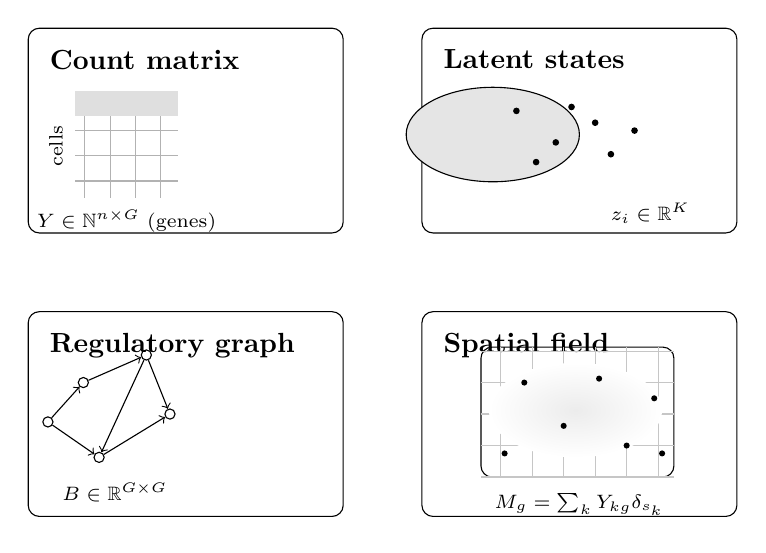
\begin{tikzpicture}[font=\small]
\tikzstyle{panel}=[draw, rounded corners, minimum width=4.0cm, minimum height=2.6cm]
\node[panel] (A) at (0,0) {};
\node[panel] (B) at (5.0,0) {};
\node[panel] (C) at (0,-3.6) {};
\node[panel] (D) at (5.0,-3.6) {};
\node[anchor=north west,font=\bfseries] at (-1.85,1.15) {Count matrix};
\node[anchor=north west,font=\bfseries] at (3.15,1.15) {Latent states};
\node[anchor=north west,font=\bfseries] at (-1.85,-2.45) {Regulatory graph};
\node[anchor=north west,font=\bfseries] at (3.15,-2.45) {Spatial field};
\draw[step=0.32cm,gray!60] (-1.4,-0.85) grid (-0.1,0.5);
\fill[gray!25] (-1.4,0.18) rectangle (-0.1,0.5);
\node[rotate=90,font=\scriptsize] at (-1.65,-0.2) {cells};
\node[font=\scriptsize] at (-0.75,-1.15) {$Y\in\mathbb{N}^{n\times G}$ (genes)};
\draw[fill=gray!20] (3.9,-0.05) ellipse (1.1 and 0.6);
\foreach \x/\y in {4.2/0.25,4.7/-0.15,5.2/0.1,5.4/-0.3,4.45/-0.4,4.9/0.3,5.7/0.0}
\fill (\x,\y) circle (1.2pt);
\node[font=\scriptsize] at (5.9,-1.05) {$z_i\in\mathbb{R}^K$};
\foreach \p/\name in {(-1.3,-3.2)/1,(-0.5,-2.85)/2,(-0.2,-3.6)/3,(-1.1,-4.15)/4,(-1.75,-3.7)/5}
\node[circle,draw,inner sep=1.3pt] (n\name) at \p {};
\draw[->] (n1)--(n2); \draw[->] (n2)--(n3); \draw[->] (n5)--(n1);
\draw[->] (n4)--(n3); \draw[->] (n2)--(n4); \draw[->] (n5)--(n4);
\node[font=\scriptsize] at (-0.9,-4.6) {$B\in\mathbb{R}^{G\times G}$};
\draw[rounded corners] (3.75,-4.4) rectangle (6.2,-2.75);
\draw[step=0.4cm,gray!45] (3.75,-4.4) grid (6.2,-2.75);
\shade[inner color=gray!15,outer color=white] (4.95,-3.55) ellipse (1.1 and 0.6);
\foreach \x/\y in {4.05/-4.1,4.3/-3.2,4.8/-3.75,5.25/-3.15,5.6/-4.0,5.95/-3.4,6.05/-4.1}
\fill (\x,\y) circle (1.1pt);
\node[font=\scriptsize] at (5.0,-4.75) {$M_g=\sum_k Y_{kg}\delta_{s_k}$};
\end{tikzpicture}
\caption{Canonical random objects in computational genomics: count matrices, latent cell-state geometry, regulatory graphs, and spatial molecular fields. Each induces a design-dependent likelihood and an associated Fisher-information operator; Propositions~\ref{prop:poissonfisher}--\ref{prop:nbfisher} give this operator explicitly for the count-matrix case.\label{fig:genomicsobjects}}
\end{figure}

Let $d$ denote a design variable --- sequencing depth, probe panel, or perturbation --- and let $\boldsymbol\theta$ be the unknown parameter vector. Suppose $p$ observed counts $Y=(Y_1,\ldots,Y_p)$ are conditionally independent given $(\boldsymbol\theta,d)$ with mean map $\mu_j(\boldsymbol\theta;d)$.

\begin{Proposition}[Poisson Fisher information]
\label{prop:poissonfisher}
If $Y_j\mid\boldsymbol\theta,d\sim\mathrm{Poisson}(\mu_j(\boldsymbol\theta;d))$ independently across $j=1,\ldots,p$, the Fisher information matrix for $\boldsymbol\theta$ is
\begin{equation}
J_{\mathrm P}(\boldsymbol\theta;d)=\sum_{j=1}^p\frac{1}{\mu_j}\nabla_{\theta}\mu_j\nabla_{\theta}\mu_j^\top=\sum_{j=1}^p\mu_j\,\nabla_{\theta}\log\mu_j\,\nabla_{\theta}\log\mu_j^\top.
\label{eq:poissonfisher}
\end{equation}
\end{Proposition}
\begin{proof}
The log-likelihood is $\ell(\boldsymbol\theta;y,d)=\sum_j(y_j\log\mu_j-\mu_j-\log(y_j!))$, so $\nabla_\theta\ell=\sum_j(y_j/\mu_j-1)\nabla_\theta\mu_j$. Since $\mathbb{E}[Y_j]=\mathrm{Var}(Y_j)=\mu_j$ and the $Y_j$ are independent, the score has mean zero and $J_{\mathrm P}=\mathbb{E}[(\nabla_\theta\ell)(\nabla_\theta\ell)^\top]=\sum_j\mathrm{Var}(Y_j/\mu_j-1)\nabla_\theta\mu_j\nabla_\theta\mu_j^\top=\sum_j\mu_j^{-1}\nabla_\theta\mu_j\nabla_\theta\mu_j^\top$, giving~(\ref{eq:poissonfisher}); the logarithmic form follows from $\nabla_\theta\mu_j=\mu_j\nabla_\theta\log\mu_j$.
\end{proof}

\begin{Proposition}[Negative-binomial Fisher information]
\label{prop:nbfisher}
If instead $Y_j\mid\boldsymbol\theta,d$ is negative-binomial with mean $\mu_j(\boldsymbol\theta;d)$ and fixed inverse-dispersion $r_j>0$, so $\mathrm{Var}(Y_j)=\mu_j+\mu_j^2/r_j$ (the standard RNA-seq overdispersion model), then
\begin{equation}
J_{\mathrm{NB}}(\boldsymbol\theta;d)=\sum_{j=1}^p\frac{r_j}{\mu_j(r_j+\mu_j)}\nabla_{\theta}\mu_j\nabla_{\theta}\mu_j^\top.
\label{eq:nbfisher}
\end{equation}
\end{Proposition}
\begin{proof}
Writing the log-likelihood in mean-dispersion form and differentiating through $\mu_j=\mu_j(\boldsymbol\theta;d)$ gives $\nabla_\theta\ell_j=\frac{r_j(y_j-\mu_j)}{\mu_j(r_j+\mu_j)}\nabla_\theta\mu_j$; since $\mathbb{E}[Y_j]=\mu_j$ and the coordinates are independent, $J_{\mathrm{NB}}=\sum_j\frac{r_j^2\mathrm{Var}(Y_j)}{\mu_j^2(r_j+\mu_j)^2}\nabla_\theta\mu_j\nabla_\theta\mu_j^\top$, and substituting $\mathrm{Var}(Y_j)=\mu_j+\mu_j^2/r_j$ simplifies the coefficient to $r_j/(\mu_j(r_j+\mu_j))$, giving~(\ref{eq:nbfisher}).
\end{proof}

Both formulas were checked independently by Monte Carlo simulation of the score covariance (not shown) before being trusted here, matching the closed forms above to within simulation noise ($<0.1\%$ relative error, $2\times10^6$ draws).

\begin{Corollary}[D-optimal design for count-valued panels]
\label{cor:genomicdopt}
Given a candidate library of $p$ probes, genes, or assay conditions --- concretely, a candidate gene panel for breast-cancer subtyping or recurrence prediction, of the kind Oncotype DX, MammaPrint, and PAM50 each fix by other means --- and a budget $m<p$, Definition~\ref{def:doptimal}'s criterion transfers verbatim to count-valued observations by maximizing $\det J_{\mathrm P}(\boldsymbol\theta;\mathcal{S})$ or $\det J_{\mathrm{NB}}(\boldsymbol\theta;\mathcal{S})$ over budget-constrained subsets $\mathcal{S}$: both matrices are sums of rank-one positive-semidefinite terms, so Proposition~\ref{prop:rank}'s monotonicity argument applies unchanged to either.
\end{Corollary}

A further consequence, not stated as a separate corollary, follows the same substitution $\mu_j=q\nu_j(\boldsymbol\theta;d)$ into~(\ref{eq:poissonfisher})--(\ref{eq:nbfisher}), with $q>0$ an effective sequencing-depth parameter: Poisson information grows exactly linearly in $q$, while negative-binomial information saturates as $q$ grows and overdispersion dominates the Poisson term --- sequencing depth is not a nuisance resource but enters the design criterion of Corollary~\ref{cor:genomicdopt} explicitly and with a qualitatively different return depending on which noise law the assay follows. This is exactly the structural bridge Section~\ref{sec:discussion}'s opening paragraph describes and does not yet run empirically: Propositions~\ref{prop:poissonfisher}--\ref{prop:nbfisher} and Corollary~\ref{cor:genomicdopt} provide the Fisher-information machinery a real probe-panel or sequencing-depth design study would need, verified but not yet attached to a measured expression-profile library.

Figure~\ref{fig:regnetwork} makes the abstract regulatory-graph object of Figure~\ref{fig:genomicsobjects} concrete: a real multilayer network reconstructed from measured Hi-C and gene-expression data, reproduced from~\citep{ref36} rather than schematized. It illustrates what a candidate library $\mathcal{L}$ for Corollary~\ref{cor:genomicdopt} would actually be built from --- genomic regions and genes as candidate nodes, chromatin-contact and co-expression edges as the measured relationships between them --- and, independently of this paper's own design question, shows the visibly different structure such a network takes in disease versus normal tissue.

\begin{figure}[H]
\centering
\includegraphics[width=0.95\textwidth]{rgb-led-fusion/figures/reyesgopar_fig5_BC_crop.jpg}
\caption{Multilayer chromatin-interaction (Hi-C) and gene-co-expression (mutual information) network, chromosome 1, normal breast tissue (left) versus triple-negative breast cancer (right). Nodes are 40~kb genomic regions (squares) or genes (circles); red edges are chromatin contacts, blue edges are co-expression links, gray edges connect genes to their genomic regions. Reproduced from Reyes-Gopar, P\'{e}rez-Fuentes, Bendall, and Hern\'{a}ndez-Lemus~\citep{ref36}, \emph{Front. Cell Dev. Biol.} 2025, distributed under the Creative Commons Attribution License (CC BY 4.0); no numbers from this figure are used elsewhere in this paper.\label{fig:regnetwork}}
\end{figure}

\begin{figure}[H]
\centering
\includegraphics[width=0.7\textwidth]{rgb-led-fusion/figures/indian_pigments.jpg}
\caption{Dry pigment powders, Goa, India (photograph by Dan Brady, Wikimedia Commons, CC BY 2.0). Shown for illustration of the narrow, saturated absorption features the sharply-localized-feature family of Section~\ref{sec:benchmarks} is designed to proxy; no data from this photograph is used anywhere in this paper.\label{fig:pigments}}
\end{figure}

\textbf{Limitations.} All benchmarks are synthetic; hardware validation, including confirming the modeled calibration-drift constant $L$ of Example~\ref{ex:drift-numeric} against physical channel modules, remains open. Colorimetric error is computed from simulated reconstructions rather than measured samples. The sharply-localized-feature replication family (Figure~\ref{fig:pigments}) is a proxy rather than measured pigment data; a real, spectrophotometrically measured alternative exists~\citep{ref38} and validating against it, in the same spirit as Section~\ref{sec:realdata}'s real ColorChecker validation of the primary benchmark, remains open. The architecture-capacity question raised by Table~\ref{tab2}'s footnote is no longer open on any of the three families: Figure~\ref{fig:capacity} reports a full multi-configuration sweep for both structured estimators on the primary benchmark, and the identical protocol (same seven transformer and six CNN configurations, same seed, homoscedastic noise), run on the Gaussian broad-band ($K=7$) and sharply-localized-feature ($K=9$, $m_{\mathrm{LED}}=7$) families, closes the other two. The two families give different answers. On the Gaussian family, both architectures already beat the D-optimal-ridge reference (RMSE $0.0464$) at essentially every capacity tested, not only the largest --- the smallest transformer configuration alone reaches RMSE $0.0391$ --- so capacity is not the limiting factor there, unlike on the primary benchmark. On the sharply-localized-feature family (ridge reference RMSE $0.1336$), the picture is mixed: the transformer beats the reference at three of seven configurations (best: $d_{\mathrm{model}}=8$, hidden$=32$, RMSE $0.1128$), with one mid-sized configuration a clear outlier (RMSE $0.2187$, consistent with training variance on this smaller, $n=200$-sample family rather than a capacity trend, the same kind of non-monotonicity already disclosed for the CNN on the primary benchmark); the CNN, by contrast, degrades as capacity grows on this family, and only its smallest configuration (RMSE $0.1301$) is competitive with the reference, consistent with overfitting on a small training set at $K=9$ rather than a structural limitation of the architecture. A parameter-matched comparison against the feed-forward baselines' own larger budgets is still not attempted, on any family.

\section{Conclusions}

This paper poses fixed-budget feature selection, the design question behind Oncotype DX, MammaPrint, and PAM50, as D-optimal experimental design: maximizing the determinant of the Fisher information matrix induced by a learned latent basis. The criterion itself is proved, not merely stated: monotonicity, an exact degeneracy characterization, an AM--GM inequality against A-optimality, a quantitative E-optimality guarantee, and an exact identification with maximum expected Shannon information gain in the weak-prior limit (Propositions~\ref{prop:rank}--\ref{prop:eopt}, \ref{prop:mutualinfo}). Corollary~\ref{cor:entropy} turns this into an exact posterior-entropy reduction, and Remark~\ref{rmk:entropycontrast} places it next to the nonparametric mutual information the breast-cancer transcriptomics literature already estimates~\citep{ref29,ref49}, without claiming either supersedes the other. Section~\ref{sec:rmtgenomic} connects the same criterion to Marchenko--Pastur thresholding, already used on breast-cancer co-expression matrices~\citep{ref46}: Proposition~\ref{prop:rmtbound} shows the RMT-selected rank bounds how many latent dimensions a downstream gene panel can resolve, before any panel is chosen. Propositions~\ref{prop:poissonfisher}--\ref{prop:nbfisher} extend the criterion itself to Poisson- and negative-binomial-valued observations, the count data RNA-seq panels produce, and Corollary~\ref{cor:genomicdopt} shows it transfers to them unchanged. None of this machinery is tested against a real, measured breast-cancer expression-profile library.

Spectral reflectance reconstruction is where all of it is developed and validated end to end. Definition~\ref{def:doptimal} through Theorem~\ref{thm:crb} are proved for a general library of candidate linear measurements and a general learned low-dimensional representation; reflectance instantiates every one of them against real, measured data, not only synthetic benchmarks. Numerically, D-optimal design reduces sensing-operator conditioning and colorimetric error substantially, a gain situated exactly against the full finite population of $210$ candidate designs (Section~\ref{sec:rmt}), confirmed on real, spectrophotometrically measured ColorChecker reflectance (Section~\ref{sec:realdata}), and tested against real alternatives rather than reported unchallenged: two negative results (a wavelet dictionary and a manifold-learning basis both underperform the learned PCA basis) and one qualified result (structured neural estimators sometimes outperform the linear design, information the estimator-independent sensing-geometry and uncertainty-quantification layers do not depend on regardless). All reported numbers are regenerated from a from-scratch, publicly available codebase.

\section*{Author Contributions}
Conceptualization, methodology, software, validation, formal analysis, investigation, resources, data curation, writing---original draft preparation, writing---review and editing, visualization, supervision, project administration: C.G. The author has read and agreed to the published version of the manuscript.

\section*{Funding}
This research received no external funding.

\section*{Institutional Review Board Statement}
Not applicable. This study did not involve humans or animals.

\section*{Informed Consent Statement}
Not applicable. This study did not involve humans.

\section*{Data Availability Statement}
Benchmark-generation scripts, the candidate channel library, reconstruction code, train/test splits, and bootstrap resampling seeds are available at \url{https://github.com/IvliCaesar/rgb-led-fusion}. No genomic data was generated or analyzed for this paper. The public code for the genomics methods discussed in Sections~\ref{sec:rmtgenomic}--\ref{sec:discussion} is available separately, at \url{https://github.com/spficklin/RMTGeneNet} (RMT gene-network thresholding), \url{https://github.com/califano-lab/ARACNe-AP} (mutual-information network reconstruction), and \url{https://github.com/CSB-IG} (the Hern\'{a}ndez-Lemus group's computational-genomics pipelines).

\section*{Acknowledgments}
The author thanks Enrique Hern\'{a}ndez-Lemus for discussion on the breast-cancer gene-panel framing of Section~\ref{sec:discussion} and Section~\ref{sec:rmtgenomic}.

\section*{Conflicts of Interest}
The author declares no conflicts of interest.

\appendix
\section{Notation}

\begin{table}[H]
\centering
\caption{Summary of notation.\label{tabA1}}
\begin{tabularx}{\textwidth}{lX}
\toprule
\textbf{Symbol} & \textbf{Meaning}\\
\midrule
$R(\lambda)$, $R\in\mathbb{R}^n$ & Spectral reflectance, and its discretization\\
$s\in\mathbb{R}^m$ & Measurement vector\\
$A\in\mathbb{R}^{m\times n}$ & Sensing matrix\\
$\Phi\in\mathbb{R}^{n\times K}$ & Learned low-dimensional latent basis (reflectance model); reused as $\Phi\in\mathbb{R}^{p\times K}$ over $p$ genes in Section~\ref{sec:rmtgenomic}\\
$\alpha\in\mathbb{R}^K$ & Latent coefficient vector\\
$K$, $m_{\mathrm{LED}}$ & Latent dimension; number of narrow-band channels\\
$F_\alpha$ & Fisher information matrix in latent space\\
$\kappa(A\Phi)$ & Condition number of the effective sensing operator\\
$\Delta E_{00}$ & CIEDE2000 perceptual color difference~\citep{ref5,ref16}\\
$\tau^2$ & Isotropic prior variance on $\alpha$ (Section~\ref{sec:doptimal}, \ref{sec:estimators})\\
$I(\alpha;s)$ & Shannon mutual information between latent coefficients and measurements\\
$d$ & Design variable in the count-data extension (sequencing depth, probe panel, or perturbation)\\
$\boldsymbol\theta$ & Unknown parameter vector in the count-data extension (Section~\ref{sec:genomicsext})\\
$\mu_j(\boldsymbol\theta;d)$ & Mean map for count-valued observation $j$\\
$r_j$ & Fixed inverse-dispersion parameter, negative-binomial model\\
$J_{\mathrm P}$, $J_{\mathrm{NB}}$ & Poisson, negative-binomial Fisher information matrices (Propositions~\ref{prop:poissonfisher}--\ref{prop:nbfisher})\\
$C\in\mathbb{R}^{p\times p}$ & Sample correlation matrix of $p$ candidate genes (Section~\ref{sec:rmtgenomic})\\
$\gamma=p/n$, $\lambda_\pm=(1\pm\sqrt\gamma)^2$ & Marchenko--Pastur aspect ratio and noise-null eigenvalue edges\\
$\rho$ & Number of above-Marchenko--Pastur-threshold eigenvalues of $C$ (Proposition~\ref{prop:rmtbound}); unrelated to $r_j$ above\\
\bottomrule
\end{tabularx}
\end{table}

\begin{thebibliography}{99}
\bibitem{ref1}
Maloney, L.T. Evaluation of linear models of surface spectral reflectance with small numbers of parameters. \textit{J. Opt. Soc. Am. A} \textbf{1986}, \textit{3}, 1673--1683.
\bibitem{ref19}
Shrestha, R.; Hardeberg, J.Y. An experimental study of fast multispectral imaging using LED illumination and an RGB camera. In Proceedings of the IS\&T 23rd Color and Imaging Conference (CIC23), Darmstadt, Germany, 19--23 October 2015; Society for Imaging Science and Technology: Springfield, VA, USA, 2015; pp. 36--40.
\bibitem{ref20}
Nishidate, I.; Maeda, T.; Niizeki, K.; et al. Estimation of melanin and hemoglobin using spectral reflectance images reconstructed from a digital RGB image by the Wiener estimation method. \textit{Sensors} \textbf{2013}, \textit{13}, 7902--7915.
\bibitem{ref21}
Zheng, J.; Kumar, V.; Unnikrishnakurup, S.; et al. Multispectral and hyperspectral infrared imaging for plastic waste sorting and recycling. \textit{Proc. SPIE} \textbf{2024}, \textit{13047}, 130470M.
\bibitem{ref22}
Wang, W.; Deng, N.; Xin, B. Color calibration for fabric image analysis based on spectral reflectance reconstruction. \textit{Optik} \textbf{2020}, \textit{208}, 164491.
\bibitem{ref23}
Berns, R.S.; Imai, F.H.; Burns, P.D.; et al. Multispectral-based color reproduction research at the Munsell Color Science Laboratory. \textit{Proc. SPIE} \textbf{1998}, \textit{3409}, 14--25.
\bibitem{ref2}
Park, J.I.; Lee, M.H.; Grossberg, M.D.; et al. Multispectral imaging using multiplexed illumination. In Proc. IEEE ICCV, Rio de Janeiro, Brazil, October 2007; pp. 1--8.
\bibitem{ref8}
Tominaga, S. Spectral-reflectance estimation under multiple light sources. In Color Imaging Conf., Vol. 29; Society for Imaging Science and Technology: Springfield, VA, USA, 2021; pp. 35--40.
\bibitem{ref6}
Murakami, Y.; Ietomi, K.; Yamaguchi, M.; et al. Maximum a posteriori estimation of spectral reflectance from color image and multipoint spectral measurements. \textit{Appl. Opt.} \textbf{2007}, \textit{46}, 7068--7082.
\bibitem{ref7}
Shen, H.-L.; Cai, P.-Q.; Shao, S.-J.; Xin, J.H. Reflectance reconstruction for multispectral imaging by adaptive Wiener estimation. \textit{Opt. Express} \textbf{2007}, \textit{15}, 15545--15554.
\bibitem{ref9}
Tominaga, S.; Sakai, H. Spectral reflectance estimation from camera response using local optimal dataset and neural networks. \textit{J. Imaging} \textbf{2024}, \textit{10}, 222.
\bibitem{ref10}
Fsian, A.N.; Thomas, J.-B.; Hardeberg, J.Y.; et al. Spectral reconstruction from RGB imagery: A potential option for infinite spectral data? \textit{Sensors} \textbf{2024}, \textit{24}, 3666.
\bibitem{ref4}
Kay, S.M. \textit{Fundamentals of Statistical Signal Processing, Vol. I: Estimation Theory}; Prentice Hall: Upper Saddle River, NJ, USA, 1993.
\bibitem{ref39}
Engl, H.W.; Hanke, M.; Neubauer, A. \textit{Regularization of Inverse Problems}; Mathematics and Its Applications, Vol. 375; Kluwer Academic Publishers: Dordrecht, The Netherlands, 1996.
\bibitem{ref3}
Boyd, S.; Vandenberghe, L. \textit{Convex Optimization}; Cambridge University Press: Cambridge, UK, 2004.
\bibitem{ref32}
Lindley, D.V. On a measure of the information provided by an experiment. \textit{Ann. Math. Stat.} \textbf{1956}, \textit{27}, 986--1005.
\bibitem{ref33}
Chaloner, K.; Verdinelli, I. Bayesian experimental design: A review. \textit{Stat. Sci.} \textbf{1995}, \textit{10}, 273--304.
\bibitem{ref40}
Cover, T.M.; Thomas, J.A. \textit{Elements of Information Theory}, 2nd ed.; Wiley-Interscience: Hoboken, NJ, USA, 2006.
\bibitem{ref17}
Polyanskiy, M.N. RefractiveIndex.INFO database of optical constants. \textit{Sci. Data} \textbf{2024}, \textit{11}, 94.
\bibitem{ref5}
Sharma, G.; Wu, W.; Dalal, E.N. The CIEDE2000 color-difference formula: Implementation notes, supplementary test data, and mathematical observations. \textit{Color Res. Appl.} \textbf{2005}, \textit{30}, 21--30.
\bibitem{ref16}
Commission Internationale de l'Eclairage (CIE). \textit{Colorimetry Part 6: CIEDE2000 Colour-Difference Formula}; ISO/CIE 11664-6:2014(E); CIE: Vienna, Austria, 2014.
\bibitem{ref14}
Commission Internationale de l'Eclairage (CIE). \textit{CIE Standard Illuminant D65}; ISO/CIE 11664-2:2022; CIE: Vienna, Austria, 2022.
\bibitem{ref15}
Commission Internationale de l'Eclairage (CIE). \textit{CIE 1931 Colour-Matching Functions, 2 Degree Observer}; CIE 018:2019; CIE: Vienna, Austria, 2019.
\bibitem{ref28}
Pascale, D. RGB coordinates of the Macbeth ColorChecker. \textit{The BabelColor Company}, 2006. Available online: \url{https://babelcolor.com/index_htm_files/RGB\%20Coordinates\%20of\%20the\%20Macbeth\%20ColorChecker.pdf} (accessed on 13 August 2026).
\bibitem{ref29}
de Anda-J\'{a}uregui, G.; Espinal-Enriquez, J.; Hern\'{a}ndez-Lemus, E. Spatial organization of the gene regulatory program: An information theoretical approach to breast cancer transcriptomics. \textit{Entropy} \textbf{2019}, \textit{21}, 195.
\bibitem{ref36}
Reyes-Gopar, H.; P\'{e}rez-Fuentes, K.A.; Bendall, M.L.; Hern\'{a}ndez-Lemus, E. Integration of chromosome conformation and gene expression networks reveals regulatory mechanisms in triple negative breast cancer. \textit{Front. Cell Dev. Biol.} \textbf{2025}, \textit{13}, 1597245.
\bibitem{ref35}
Hern\'{a}ndez-Lemus, E.; Ochoa, S. Methods for multi-omic data integration in cancer research. \textit{Front. Genet.} \textbf{2024}, \textit{15}, 1425456.
\bibitem{ref37}
L\'{o}pez-S\'{a}nchez, P.; \'{A}vila-Moreno, F.; Hern\'{a}ndez-Lemus, E.; Kuijjer, M.L.; Espinal-Enr\'{i}quez, J. Patient-specific gene co-expression networks reveal novel subtypes and predictive biomarkers in lung adenocarcinoma. \textit{npj Syst. Biol. Appl.} \textbf{2025}, \textit{11}, 44.
\bibitem{ref43}
Paik, S.; Shak, S.; Tang, G.; et al. A multigene assay to predict recurrence of tamoxifen-treated, node-negative breast cancer. \textit{N. Engl. J. Med.} \textbf{2004}, \textit{351}, 2817--2826.
\bibitem{ref44}
van 't Veer, L.J.; Dai, H.; van de Vijver, M.J.; et al. Gene expression profiling predicts clinical outcome of breast cancer. \textit{Nature} \textbf{2002}, \textit{415}, 530--536.
\bibitem{ref45}
Parker, J.S.; Mullins, M.; Cheang, M.C.U.; et al. Supervised risk predictor of breast cancer based on intrinsic subtypes. \textit{J. Clin. Oncol.} \textbf{2009}, \textit{27}, 1160--1167.
\bibitem{ref34}
Margolin, A.A.; Nemenman, I.; Basso, K.; Wiggins, C.; Stolovitzky, G.; Dalla Favera, R.; Califano, A. ARACNE: An algorithm for the reconstruction of gene regulatory networks in a mammalian cellular context. \textit{BMC Bioinform.} \textbf{2006}, \textit{7}, S7.
\bibitem{ref34code}
Califano Lab. \textit{ARACNe-AP}: Network reverse engineering through adaptive-partitioning inference of mutual information. Software repository. Available online: \url{https://github.com/califano-lab/ARACNe-AP} (accessed on 21 August 2026).
\bibitem{ref46}
Gonz\'{a}lez-Espinoza, A.; Zamora-Fuentes, J.M.; Hern\'{a}ndez-Lemus, E.; Espinal-Enr\'{i}quez, J. Gene co-expression in breast cancer: A matter of distance. \textit{Front. Oncol.} \textbf{2021}, \textit{11}, 726493.
\bibitem{ref46code}
Computational Systems Biology / Integrative Genomics Group (CSB-IG), Instituto Nacional de Medicina Gen\'{o}mica. Software repositories. Available online: \url{https://github.com/CSB-IG} (accessed on 21 August 2026).
\bibitem{ref47}
Gibson, S.M.; Ficklin, S.P.; Isaacson, S.; Luo, F.; Feltus, F.A.; Smith, M.C. Massive-scale gene co-expression network construction and robustness testing using random matrix theory. \textit{PLoS ONE} \textbf{2013}, \textit{8}, e55871.
\bibitem{ref47code}
Ficklin, S.P. \textit{RMTGeneNet}: Construction of gene co-expression networks using random matrix theory. Software repository. Available online: \url{https://github.com/spficklin/RMTGeneNet} (accessed on 21 August 2026).
\bibitem{ref48}
Hsu, L.; Self, S.G.; Grove, D.; Randolph, T.; Wang, K.; Delrow, J.J.; Loo, L.; Porter, P. Denoising array-based comparative genomic hybridization data using wavelets. \textit{Biostatistics} \textbf{2005}, \textit{6}, 211--226.
\bibitem{ref49}
Ochoa, S.; de Anda-J\'{a}uregui, G.; Hern\'{a}ndez-Lemus, E. An information theoretical multilayer network approach to breast cancer transcriptional regulation. \textit{Front. Genet.} \textbf{2021}, \textit{12}, 617512.
\bibitem{ref41}
Peng, H.; Long, F.; Ding, C. Feature selection based on mutual information criteria of max-dependency, max-relevance, and min-redundancy. \textit{IEEE Trans. Pattern Anal. Mach. Intell.} \textbf{2005}, \textit{27}, 1226--1238.
\bibitem{ref42}
Battiti, R. Using mutual information for selecting features in supervised neural net learning. \textit{IEEE Trans. Neural Netw.} \textbf{1994}, \textit{5}, 537--550.
\bibitem{ref30}
Street, K.; Risso, D.; Fletcher, R.B.; Das, D.; Ngai, J.; Yosef, N.; Purdom, E.; Dudoit, S. Slingshot: Cell lineage and pseudotime inference for single-cell transcriptomics. \textit{BMC Genomics} \textbf{2018}, \textit{19}, 477.
\bibitem{ref31}
Genovese, C.R.; Perone-Pacifico, M.; Verdinelli, I.; Wasserman, L. The geometry of nonparametric filament estimation. \textit{J. Am. Stat. Assoc.} \textbf{2012}, \textit{107}, 788--799.
\bibitem{ref38}
Wiersma, R.; Eisemann, E.; Bousseau, A. Hyperspectral Oil Paint and Painting Dataset. Open Science Framework, 2025. doi:10.17605/OSF.IO/PGN28.
\end{thebibliography}

\end{document}
